% Farbkarte TU Darmstadt: http://www.webteam.tu-darmstadt.de/media/webteam_wissensdatenbank/artikel_1/farbkarte_TU_Darmstadt.png
\documentclass[nochapterpage,nopartpage,noheadingspace,numbersubsubsec,bigchapter,colorback,accentcolor=tud9c,10pt]{tudreport}
\usepackage[ngerman,english]{babel}

\usepackage[stable]{footmisc}
\usepackage[ngerman,english]{hyperref}

\usepackage{longtable}
\usepackage{multirow}
\usepackage{booktabs}

% Custom packages
\usepackage{wrapfig}
\usepackage{etoolbox}
\usepackage{multicol}
\usepackage{listings}

\lstset{
    breaklines=true,
    postbreak=\raisebox{0ex}[0ex][0ex]{\ensuremath{\color{red}\hookrightarrow\space}}
}

% Reset chapter counter after introducing a new part and start chapters on the same page
\makeatletter
\@addtoreset{chapter}{part}
\patchcmd{\scr@startchapter}{\if@openright\cleardoublepage\else\clearpage\fi}{}{}{}
\makeatother

\hypersetup{%
  pdftitle={Internet Praktikum TK Documentation},
  pdfauthor={M. Schanz},
  pdfsubject={Project Documentation},
  pdfview=FitH,
  pdfstartview=FitV
}

%%% Zum Tester der Marginalien %%%
  \newif\ifTUDmargin\TUDmarginfalse
  %%% Wird der Folgende Zeile einkommentiert,
  %%% werden Marginalien gesetzt.
  % \TUDmargintrue
  \ifTUDmargin\makeatletter
    \TUD@setmarginpar{2}
  \makeatother\fi
%%% ENDE: Zum Tester der Marginalien %%%

\newlength{\longtablewidth}
\setlength{\longtablewidth}{0.7\linewidth}
\addtolength{\longtablewidth}{-\marginparsep}
\addtolength{\longtablewidth}{-\marginparwidth}

\title{Internet Praktikum TK 2016\\ Conference Management System\\ Team Whisky}
\subtitle{Auel, Tarek,\\ Sahin, Huzeyfe\\ Schanz, Markus}


\begin{document}
\maketitle
\tableofcontents
%\listoffigures
%\addcontentsline{toc}{chapter}{\listfigurename}



\part{User Documentation}
\label{part:user}
    % linewidth/textwidth: 17.49751cm = 497.92325pt
    % Good screenshot ratio: 1,7066 (=> 1280×750)

  \chapter{Introduction}
  \label{ch:user:intro}

    \texttt{TKonference} is a web-based conference management system that offers all required features for managing attendees, authors, reviewers, and chair(s) of a conference. The application is open-source and highly extendable. If you are a server administrator who wants to install this software as a self-hosted solution, please refer to appendix~\ref{ch:appendix:setup} for the required prerequisites and installation instructions. If you are a developer who wants to extend the application, please refer to part~\ref{part:tech} of this documentation which provides an overview of the software's architecture and implementation.

    This part of the documentation is meant as a guide for users of the application. It describes the usage of the application and its provided features. The remainder of the guide is divided into five sections, each dedicated to one of the following user roles, respectively:
        \begin{itemize}
            \setlength\itemsep{0em}
            \item \texttt{User}: Basically, a user is someone who is visiting the web application with a web browser.%
            \footnote{Strictly speaking, a user is someone who authenticated himself against the application with a valid username and password. This distinction is only relevant if you are a developer (see~part~\ref{part:tech}, section~\ref{sec:tech:implementation:acl:roles}).}
            This is the most restricted account type which is only allowed to perform basic actions (see chapter~\ref{ch:user:user}).
            \item \texttt{Attendee}: An attendee is a user who is actively participating at a specific conference. A user can become an attendee of a conference by joining it (see chapter~\ref{ch:user:attendee}).
            \item \texttt{Author}: An author is an attendee of a conference who has the permission to submit a conference-relevant paper (PDF), thus applying as a speaker (see chapter~\ref{ch:user:author}).
            \item \texttt{Reviewer}: Reviewers are persons with great expertise in the research area that is targeted by the conference. They are responsible to review submitted papers of authors, i.e., provide them with feedback, and rate the  quality and relevance of the submitted paper (see chapter~\ref{ch:user:reviewer}).
            \item \texttt{Chair}: The chair is responsible for managing the conference. He has the power to name authors, reviewers, and further chairs from the list of attendees. When the review phase is over, the chair decides, based on the given reviews, which papers to approve and therefore which authors to invite as a speaker (see chapter~\ref{ch:user:chair}).
        \end{itemize}

        \begin{figure}
            \centering
            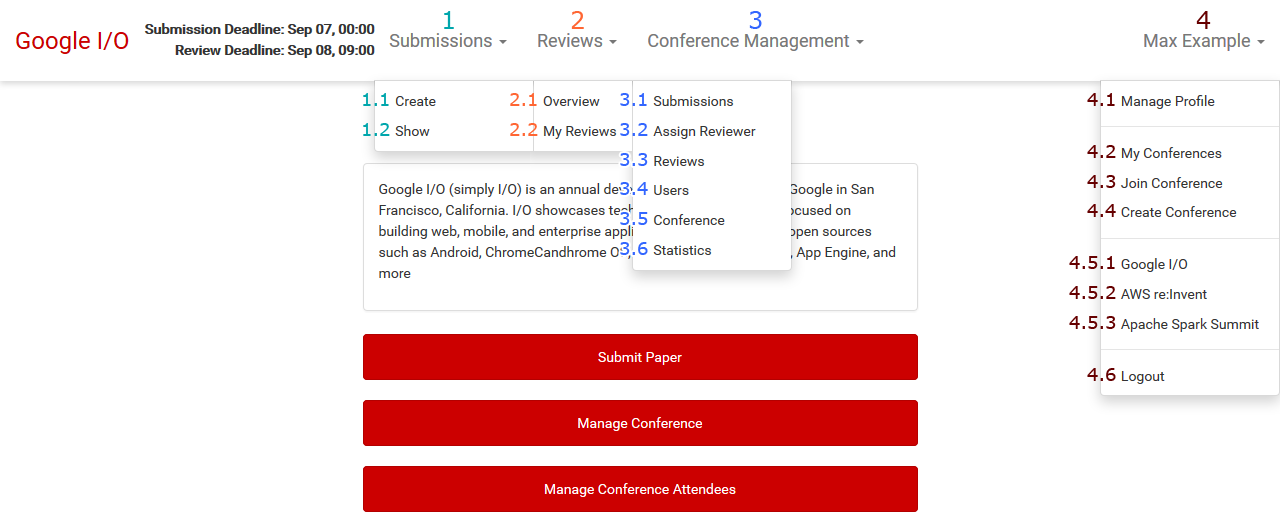
\includegraphics[width=\textwidth]{img/ui-menus}
            \caption{Application UI - Logged in, menus opened}
            \label{fig:user:intro:ui-menus}
        \end{figure}

  \chapter{User}
  \label{ch:user:user}

    The basic abilities of a user comprise of \ref{ch:user:user:register}) registering of a new account, \ref{ch:user:user:login}) log in to an account, \ref{ch:user:user:profile}) manage the profile of an account, and \ref{ch:user:user:create-conference}) create own conferences.

    For the remainder of this chapter, except for \ref{ch:user:user:register} and \ref{ch:user:user:login}, it is assumed that the user is logged in to the system and has already opened the start page of \texttt{TKonference} in a web browser (e.g. \url{http://localhost:3000}, when setup locally).

  \section{Create an Account}
  \label{ch:user:user:register}

        \begin{enumerate}
            \setlength\itemsep{0em}
            \item Click on the \texttt{Create new account} link (Figure~\ref{fig:appendix:screenshots:ui-login}).
            \item Fill out the name-, email-, username-, affiliation-, and password-fields, respectively (Figure~\ref{fig:appendix:screenshots:ui-register})
            \item Click the \texttt{Submit} button to complete the registration process.
        \end{enumerate}

    \noindent
    On success, the user is redirected to the login page.

  \section{Application Login}
  \label{ch:user:user:login}

        \begin{enumerate}
            \setlength\itemsep{0em}
            \item Fill out the username-, and password-field of the login form (Figure~\ref{fig:appendix:screenshots:ui-login}).
            \item Press the \texttt{Login} button to authenticate yourself against the system.
        \end{enumerate}

    \noindent
    On success, the user is redirected a) to his account overview (Figure~\ref{fig:appendix:screenshots:ui-account-home}), or b) to the conference overview of his default conference, in case he has set one (Figure~\ref{fig:appendix:screenshots:ui-conference-home}).

  \section{Application Logout}
  \label{ch:user:user:logout}

        \begin{enumerate}
            \setlength\itemsep{0em}
            \item Navigate to the drop-down menu located in the top right corner and open it by clicking on \texttt{<your name>} (Figure~\ref{fig:user:intro:ui-menus}, \#4)
            \item Inside the newly opened menu, click on the \texttt{Logout} link (Figure~\ref{fig:user:intro:ui-menus}, \#4.6).
        \end{enumerate}

    \noindent
    The log out operation is important whenever multiple persons have access to the computer.

  \section{Manage Profile}
  \label{ch:user:user:profile}

        \begin{enumerate}
            \setlength\itemsep{0em}
            \item Navigate to the drop-down menu located in the top right corner and open it by clicking on \texttt{<your name>} (Figure~\ref{fig:user:intro:ui-menus}, \#4)
            \item Inside the newly opened menu, click on the \texttt{Manage Profile} link (Figure~\ref{fig:user:intro:ui-menus}, \#4.1).
            \item Choose amongst the items in the top menu according to the options below (Figure~\ref{fig:appendix:screenshots:ui-manage-profile}).
            \begin{enumerate}
                \item Edit your profile (default):\\
                Adapt your profile as desired and confirm the changes by pressing the \texttt{Edit Profile} button.
                \item Change your password:\\
                Enter your new password in both fields to avoid misspelling and confirm it by pressing the \texttt{Change} button.
                \item Delete your account:\\
                Delete your account by pressing the \texttt{Delete} button. Read the displayed instructions carefully and confirm your decision by entering your username in the form field and pressing the \texttt{I understand the consequences, delete this profile} button.
            \end{enumerate}
        \end{enumerate}

  \section{List Attended Conferences}
  \label{ch:user:user:list-conferences}

        \begin{enumerate}
            \setlength\itemsep{0em}
            \item Navigate to the drop-down menu located in the top right corner and open it by clicking on \texttt{<your name>} (Figure~\ref{fig:user:intro:ui-menus}, \#4)
            \item Inside the newly opened menu, click on the \texttt{My Conferences} link (Figure~\ref{fig:user:intro:ui-menus}, \#4.2).
        \end{enumerate}

    \noindent
    This will list all conferences that the user attends, as well as some related quick links (Figure~\ref{fig:appendix:screenshots:ui-list-conferences}). In case that the user does not attend any conference, he is provided with two quick links to create a conference (\ref{ch:user:user:create-conference}), or join a conference (\ref{ch:user:attendee:join-conference}), accordingly.

  \section{Create a Conference}
  \label{ch:user:user:create-conference}

    \texttt{TKonference} is able to manage multiple conferences. All users are allowed to create their own conference which automatically makes them the chair of it.

        \begin{enumerate}
            \setlength\itemsep{0em}
            \item Navigate to the drop-down menu located in the top right corner and open it by clicking on \texttt{<your name>} (Figure~\ref{fig:user:intro:ui-menus}, \#4)
            \item Inside the newly opened menu, click on the \texttt{Create Conference} link (Figure~\ref{fig:user:intro:ui-menus}, \#4.4).
            \item Fill out the form with a conference name, description, important deadlines, and a shared secret (Figure~\ref{fig:appendix:screenshots:ui-conference-create}). This secret must be known by other users if they want to join your conference as an attendee.
        \end{enumerate}

  \section{Select a Conference}
  \label{ch:user:user:select-conference}

    Because a user is able to attend multiple conferences, he has to select an 'active' conference. The conference name, and links displayed in the header navigation bar are valid for the active conference only.

        \begin{enumerate}
            \setlength\itemsep{0em}
            \item Navigate to the drop-down menu located in the top right corner and open it by clicking on \texttt{<your name>} (Figure~\ref{fig:user:intro:ui-menus}, \#4)
            \item Inside the newly opened menu, select one of the conferences that you attend (Figure~\ref{fig:user:intro:ui-menus}, \#4.5.1, \#4.5.2, \#4.5.3).
        \end{enumerate}

    \noindent
    You are now redirected to the conference overview (Figure~\ref{fig:appendix:screenshots:ui-conference-home}). Also, the navigation bar is updated and shows the conference name and deadlines.

  \chapter{Attendee}
  \label{ch:user:attendee}

    An attendee is a user who is a member of a conference. In order to become an attendee, a user has to join a conference.

  \section{Join a Conference}
  \label{ch:user:attendee:join-conference}

        \begin{enumerate}
            \setlength\itemsep{0em}
            \item Navigate to the drop-down menu located in the top right corner and open it by clicking on \texttt{<your name>} (Figure~\ref{fig:user:intro:ui-menus}, \#4)
            \item Inside the newly opened menu, click on the \texttt{Join Conference} link (Figure~\ref{fig:user:intro:ui-menus}, \#4.3).
            \item Select the conference that you want to join from the drop down list and fill out the shared secret that you received from the chair or other attendees of the conference.
            \item Confirm by pressing the \texttt{Join Conference} button.
        \end{enumerate}

    On success you are redirected to the conference overview page (Figure~\ref{fig:appendix:screenshots:ui-conference-home}) which now also displays the joined conference.

  \chapter{Author}
  \label{ch:user:author}

    Those who attend a conference can be assigned the author role by the chair of the conference. An author is allowed to submit papers for the conference during the submission phase.

  \section{Create a Submission}
  \label{ch:user:author:create-submission}

        \begin{enumerate}
            \setlength\itemsep{0em}
            \item Navigate to the submission creation page by clicking \texttt{Submissions > Create Submission} (Figure~\ref{fig:user:intro:ui-menus}, \#1.1).
            \item You are now presented with the submission creation page (Figure~\ref{fig:appendix:screenshots:ui-submission-create}). The provided form allows you to select multiple co-authors from the list of conference attendees. The abstract field does support markdown syntax. You may provide multiple keywords for your paper. Please note that the uploaded paper must be provided as PDF.
            \item Confirm your submission by pressing the \texttt{Submit Paper} button.
        \end{enumerate}

    \noindent
    The newly created submission is automatically created as draft. You may edit the submission until it is marked as final (see next)

  \section{Edit and Delete a Submission}
  \label{ch:user:author:edit-sbumission}

        \begin{enumerate}
            \setlength\itemsep{0em}
            \item Navigate to the submission overview (Figure~\ref{fig:appendix:screenshots:ui-submission-overview}) by clicking \texttt{Submissions > Manage Submissions} (Figure~\ref{fig:user:intro:ui-menus}, \#1.2).
            \item Press the \texttt{Edit} (\texttt{Withdraw}) button to edit (delete) the corresponding submission.
        \end{enumerate}

    \noindent
    To finalize your submission, press on the \texttt{Final} switch within the submission overview. Once a submission is final, it can not be edited anymore. This allows reviewers to start the review process early on.

  \chapter{Reviewer}
  \label{ch:user:reviewer}

    Reviewers are allowed to create reviews for their assigned submissions during the review phase. A review consists of the expertise of the reviewer (1-5), the overall rating of the submitted paper (1-5), and a textual feedback for each of the following:
        \begin{multicols}{2}
        \begin{itemize}
            \item Evaluation Summary
            \item Detailed Comments
            \item Major Strong Points
            \item Major Weak Points
        \end{itemize}
        \end{multicols}

  \section{Create a Review}
  \label{ch:user:reviewer:create-review}

        \begin{enumerate}
            \setlength\itemsep{0em}
            \item Navigate to the review overview (Figure~\ref{fig:appendix:screenshots:ui-review-overview}) by clicking \texttt{Reviews > Show Reviews} (Figure~\ref{fig:user:intro:ui-menus}, \#2.1).
            \item Press the \texttt{Review} button to create/edit the corresponding review.
            \item Fill out the form accordingly (Figure~\ref{fig:appendix:screenshots:ui-review-create}).\\
            Note that all textual inputs on this page support markdown syntax.
            \item Save your review by pressing the \texttt{Submit Review} button.
        \end{enumerate}

  \chapter{Chair}
  \label{ch:user:chair}

    The chair of the conference is responsible to manage the conference by providing the submission- and review deadlines, assign author and reviewer roles to attendees and assign submissions to reviewers. He is also able to view the conference statistic page that visualizes and aggregates useful information.

    The process of listing submissions and reviews (Figure~\ref{fig:user:intro:ui-menus}, \#3.1 and \#3.2) does not require any further explanation and therefore, no dedicated section exists to explain these features. The process of managing a conference (Figure~\ref{fig:user:intro:ui-menus}, \#3.5) is equivalent to that of creating a conference which was explained previously in section~\ref{ch:user:user:create-conference}.

  \section{Assign User Roles to Attendees}
  \label{ch:user:chair:assign-roles}

    By default, members who join a conference have no privileges. The chair can empower attendees of the conference to gain the privileges of an author, reviewer, or chair which allows them to execute the actions described in chapter~\ref{ch:user:author}, \ref{ch:user:reviewer}, and \ref{ch:user:chair}, respectively.

        \begin{enumerate}
            \setlength\itemsep{0em}
            \item Navigate to the user management (Figure~\ref{fig:appendix:screenshots:ui-user-role-assignment}) by clicking \texttt{Conference Management > Assign User Roles} (Figure~\ref{fig:user:intro:ui-menus}, \#3.4).
            \item In the list of conference attendees, each user is displayed in a separate panel. Each panel contains three switches for the author, reviewer, and chair role, respectively. Click on any of the switches to toggle the user role. No further confirmation is necessary.
        \end{enumerate}

  \section{Assign Reviewer to Submissions}
  \label{ch:user:chair:assign-reviewer}

    Once an author create a submission, the chair is able to assign any number of reviewers to it. These reviewers will then have the ability to write a review for this submission (individually).

        \begin{enumerate}
            \setlength\itemsep{0em}
            \item Navigate to the review assignment page (Figure~\ref{fig:appendix:screenshots:ui-reviewer-assignment}) by clicking \texttt{Conference Management > Assign Reviewer} (Figure~\ref{fig:user:intro:ui-menus}, \#3.3).
            \item Each available submission is now displayed in its own panel. You may assign reviewers by one of the following methods:
            \begin{enumerate}
                \item \texttt{Manual assignment}: Within the individual panels, select the reviewers manually from the pre-populated drop down lists. They hold a list of all known reviewers of the conference.
                \item \texttt{Automatic assignment}: For an effortless mass-assignment of reviewers, use the \texttt{Auto Assignment} button on top of the page. It will randomly assign an equal number of reviewers to each submission (if possible). However, it wont assign reviewers to submissions of which they are a co-author.\\
                When using this function, be aware of the fact that manual assignments will be overridden.
            \end{enumerate}
            \item Click on the \texttt{Save Changes} button to confirm the assignments.
        \end{enumerate}

  \section{Statistics}
  \label{ch:user:chair:statistics}

    The statistics (Figure~\ref{fig:appendix:screenshots:ui-statistics}) are reached by navigating to the corresponding page via \texttt{Conference Management > Show Statistics} (Figure~\ref{fig:user:intro:ui-menus}, \#3.6). This page aggregates available information about the conference in five diagrams:
        \begin{itemize}
            \setlength\itemsep{0em}
            \item \texttt{User Role Distribution}:\\
            Shows the number of attendees, authors, reviewers, and chairs of a conference as a bar diagram.
            \item \texttt{Author/Submission Relationship}:\\
            A bar diagram that displays the number of total submissions and the number of total authors of these submissions.
            \item \texttt{Review Status}:\\
            Shows a doughnut diagram that visualizes the relationship between reviews in draft- and finish state.
            \item \texttt{Submissions by Affiliation}:\\
            Shows a bar diagram with the top 3 affiliations, i.e., the ones with the highest number of (co-)authors.
            \item \texttt{Submission Status}:\\
            Shows a doughnut diagram that visualizes the relationship between submissions in draft-, finish-, and approved status.
        \end{itemize}

\part{Technical Documentation}
\label{part:tech}

  \chapter{Introduction}
  \label{ch:tech:intro}

    This part of the documentation is intended for developers who want to setup the project on their local machine and contribute changes to the source code. The documentation is written such that the individual chapters can be read in arbitrary order. Each chapter is a self-contained piece of documentation. However, the software tools listed in section~\ref{sec:tech:architecture:3rd-party} are heavily used throughout the application. Therefore, the reader is advised to take a look at them before proceeding with the rest of the documentation. For further information on these tools, please refer to the individual project sites. Appendix~\ref{ch:appendix:setup} hold the instructions on how to setup the application on a local machine.

    The remainder of this documentation is structured as follows: Chapter~\ref{ch:tech:architecture} gives an insight of how the application works conceptually and provides an overview of the used software libraries. Implementation details such as authentication, authorization, etc. are covered in chapter~\ref{ch:tech:implementation}. This chapter also covers the directory structure of the project as well as important files that are involved in bootstrapping the application. Eventually, chapter~\ref{ch:tech:handson} describes the process of extending the application, i.e., how to extend the navigation bar, add a new page, etc.

  \chapter{Architecture}
  \label{ch:tech:architecture}

        \begin{figure}[!ht]
            \centering
            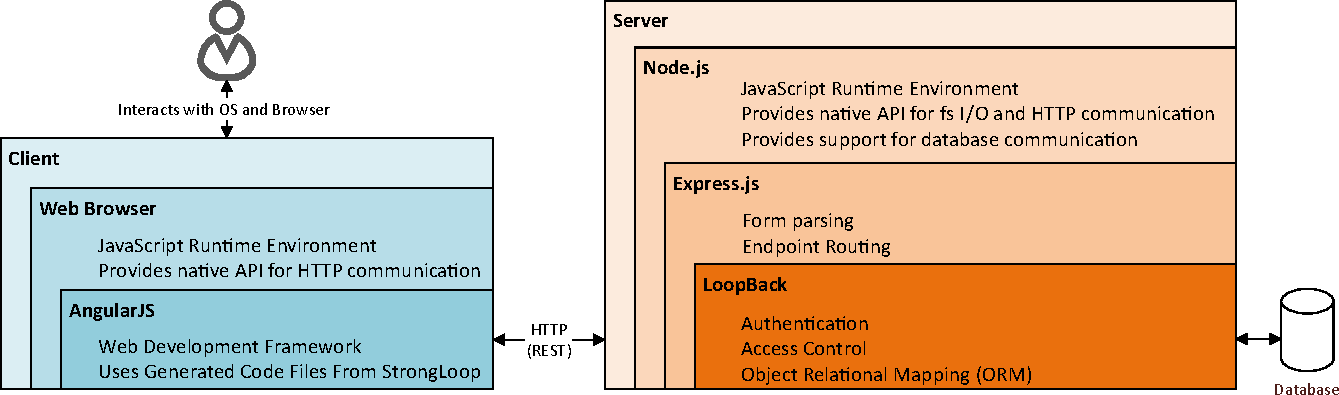
\includegraphics[width=\textwidth]{img/architecture-horizontal}
            \caption{Architecture.}
            \label{fig:tech:architecture}
        \end{figure}

        %\begin{wrapfigure}{r}{0.5\textwidth}
        %\begin{figure}
        %    \centering
        %    \includegraphics[width=0.48\textwidth]{TUDreport-fig}
        %    \caption{In curley braces.}
        %    \label{fig:client-server}
        %\end{figure}
        %\end{wrapfigure}
  \section{Overview}
  \label{sec:tech:architecture:overview}
    On a high-level view, the application follows a client-server approach. The server part of the application primarily manages the database and provides a public REST API%
    \footnote{\url{https://en.wikipedia.org/wiki/Representational_state_transfer}}
    whereas the client part runs in the browser of the user and provides an user interface (UI). The client part is responsible to translate user interactions into requests against the server API and reflect the responses in the UI.

  \section{Third Party Software}
  \label{sec:tech:architecture:3rd-party}

    As seen in figure~\ref{fig:tech:architecture}, the application utilizes third party software \& libraries in order to keep the codebase clean and allow for a productive development. This section gives an overview of the most important third party libraries \& tools that the project relies on.

  \paragraph{Node.js \& Node Package Manager}
    \emph{Node.js} is a standalone JavaScript runtime environment, i.e., it requires no web browser to execute JavaScript code.%
    \footnote{\url{https://nodejs.org/}}
    In recent years, \emph{Node.js} became very popular as it allows developers to use JavaScript for both server and client programming. It comes bundled together with its own package manager \emph{npm} which can be used to install a wide variety of third party libraries that further ease the development process.

  \paragraph{StrongLoop}
    \emph{StrongLoop} is a mandatory library on which the application is primarily build upon.%
    \footnote{\url{https://strongloop.com/}}
    This tool is able to generate code files for both server and client that can be used to manipulate a previously defined database schema. It comes bundled with a framework called \emph{LoopBack} and a library called \emph{Express.js} that is used internally to parse and route HTTP requests. It can be installed (and kept up-to-date) via \emph{npm}.

  \paragraph{Bower}
    Analogous to \emph{npm}, \emph{Bower} is a package manager for JavaScript libraries.%
    \footnote{\url{https://bower.io/}}
    However, \emph{npm} manages libraries that are required for the server part of the application (Node.js) whereas \emph{Bower} focuses on the management of libraries that are used on the client side, i.e., in the browser.

  \paragraph{AngularJS}
    AngularJS is a web application framework that eases web development by providing a model-view-controller (MVC) like architecture.%
    \footnote{\url{https://angularjs.org/}}
    The code that is generated by \emph{StrongLoop} is also targeting AngularJS.

  \chapter{Implementation}
  \label{ch:tech:implementation}

    % TODO: Introduction. This chapter covers the implementation details of the project.

  \section{Project Directory Structure}
  \label{sec:tech:implementation:dirs}

    The top level directory of the project is organized as follows:
        \begin{multicols}{4}
            \begin{itemize}
                \item /bin
                \item /client
                \item /common
                \item /doc
                \item /node\_modules
                \item /server
                \item /storage
            \end{itemize}
        \end{multicols}

  \paragraph{/}
    Besides the listed directories above, the root directory \emph{/} does contain several files worth mentioning. \emph{bower.json} and \emph{.bowerrc} are the configuration files that are automatically found and loaded by \emph{Bower}. They contain the list of dependencies and corresponding version constraints to be installed by \emph{Bower}. By renaming the \emph{db.json.default} file to \emph{db.json}, the application can be tested with some predefined seed data. The \emph{package.json} file is to \emph{npm} what \emph{bower.json} is to \emph{Bower}. The other files in the directory are either self-explaining or irrelevant for this part of the documentation.

  \paragraph{/bin}
    Contains executable scripts that are used to initialize the application database with dummy data.

  \paragraph{/client}
    Resembles the root directory that is publicly accessible through the HTTP web server, i.e., it contains all the code that is relevant for the client application.

  \paragraph{/common}
    Holds the models that describe the application database schema. These models are taken into account by \emph{StrongLoop} when generating the client- and server code files. The files inside this directory can either be edited manually (according to a specified standard) or through the \emph{StrongLoop} console line interface (see~\ref{sec:tech:implementation:strongloop:models}).

  \paragraph{/doc}
    Contains all documentation relevant files such as the documentation at hand.

  \paragraph{/node\_modules}
    This is where \emph{npm} stores downloaded modules. Besides a \emph{.gitignore} file, this directory is empty when the repository is checked out cleanly.

  \paragraph{/server}
    Contains the code that is executed inside the Node.js environment on the server side. It provides the logic to manipulate data, handles authentication and access control and also provides the public REST API.

  \paragraph{/storage}
    \emph{LoopBack}\footnote{The framework provided by \emph{StrongLoop}} manages file uploads in so-called containers. This directory contains one directory for each container and each of these hold in turn a list of files that were uploaded to the corresponding container. The directory is initially empty when the repository is checked out cleanly. It gets filled once the conference users start to submit their papers.

  \section{Entry Scripts}
  \label{sec:tech:implementation:bootstrapping}

    Entry scripts are the first step in the bootstrapping process of the application. These are somewhat comparable to the \emph{main()} method of a \emph{C++} program. Since the application runs in a distributed fashion, i.e., on a client and a server, it has entry scripts for both of them.

  \subsection{Server Application}
  \label{sec:tech:implementation:bootstrapping:server}

    As described in section~\ref{sec:tech:implementation:dirs}, the server part of the application resides inside \emph{/server}. When \emph{Node.js} is started inside the project root directory via \texttt{node .}, it executes the script \emph{server/server.js}, as defined in \emph{package.json}. Like most of the files inside \emph{server/}, this file is a slightly modified version of the \emph{LoopBack} example application%
    \footnote{\url{https://github.com/strongloop/loopback-example-passport}}. It setups some preliminary routes for \emph{Express.js} as well as configuring some middleware components, e.g., to parse form data. Eventually, the start-up routine is invoked and forwards all requests to \emph{LoopBack} which then handles the request accordingly.

    The purpose of \emph{StrongLoop} is to provide a REST API to do basic CRUD\footnote{Create/Read/Update/Delete operations on a persistent storage} operations on a predefined database schema. Since all the magic is done by \emph{StrongLoop}, a developer usually does not need to dive further into the topic of request handling etc. Everything that a developer needs to do is defining and/or extending the models inside \emph{/common/models} and \emph{StrongLoop} will take care of the rest. The process of model creation and modification is described later in section~\ref{sec:tech:implementation:strongloop:models}.

  \subsection{Web Application}
  \label{sec:tech:implementation:bootstrapping:web}

    As previously mentioned~(\ref{sec:tech:implementation:dirs}), the \emph{/client} directory is exposed through the HTTP web server. In particular, the client is eventually sending an HTTP request to the root of this directory. Because no particular file is requested by the client, the server will respond with the contents of the \emph{index.html} file.

    The \emph{index.html} file consists of a simple HTML5 skeleton which basically includes lots of CSS and JavaScript files. One of the libraries that gets included by the file is \emph{AngularJS}. Once the browser is done with parsing the page and loading all embedded JavaScript files, the \emph{AngularJS} framework is scanning for an \texttt{ng-app} attribute inside the DOM. When found, AngularJS automatically starts its bootstrap routine and eventually executes the application, which is happen to be defined inside \emph{js/app.js}. Section~\ref{sec:tech:implementation:angularjs} covers the contents of this file.

  \section{StrongLoop}
  \label{sec:tech:implementation:strongloop}

    As explained in section~\ref{sec:tech:architecture:3rd-party}, \emph{StrongLoop} is the tool that the application uses to execute CRUD operations on the database. Besides utilizing \emph{StrongLoop} as an ORM, the application makes also use of its other features such as authentication- \& session management, access control and file upload support. The application is mainly managed by the command line tool, \texttt{slc}, that comes together with \emph{StrongLoop}. It allows to generate and extend models, define access control rules, and more things. For an exhaustive description of the tool, please refer to the official documentation.\footnote{\url{https://docs.strongloop.com/display/public/LB/Command-line+reference}}

  \subsection{Creating and Updating Models}
  \label{sec:tech:implementation:strongloop:models}

    \emph{StrongLoop} does represent database tables in terms of models. A model does represent a collection of data with a given schema, e.g., a collection of users that have properties like a name, an email, a password, etc. Besides the sheer representation of data, the developer can define access rules in the model that define which data can be accessed by whom. In particular, this feature allows to restrict data-access to the owner of the data (see~\ref{sec:tech:implementation:acl:strongloop-acl}). That said, a model does also provide the methods required to retrieve, store, update and delete items of a collection.

    To update or create a model, one has to decide between two basic approaches, i.e., a guided and a manual one. The advantages and disadvantages of both approaches are described next.

  \paragraph{Guided Approach}
    In the guided approach, the user can use the command line tool of \emph{StrongLoop} to extend or create models. In particular, the tool is capable of creating models (\texttt{slc loopback:model}), add properties to an existing one (\texttt{slc loopback:property}), associate ACL\footnote{ACL stands for access control list} rules (\texttt{slc loopback:acl}) and add relations\footnote{Possible relation types are HasOne, BelongsTo, HasMany, HasManyThrough and HasAndBelongsToMany} (\texttt{slc loopback:relation}). The main advantage of this approach is that it is easy to use and does not require the knowledge of the internal configuration format. In most parts it can be used intuitively without reading the documentation.

  \paragraph{Manual Approach}
    In the manual approach, the user has to edit the model directly inside the editor. This approach is useful for advanced ACL-, property- or relation-declarations. The command line tool does only generate basic code which is not sufficient for some use cases. In these cases, the user can use a hybrid approach in which he generates the basic code with the help of the command line tool and edit it manually afterwards. Please refer to the official \emph{StrongLoop} documentation for further information regarding the model format.\footnote{\url{https://docs.strongloop.com/display/public/LB/Defining+models}}

  \subsection{File Upload}
  \label{sec:tech:implementation:strongloop:container}

    The \emph{LoopBack} framework that comes with \emph{StrongLoop} does provide the ability to persist uploaded files from users. It does so by managing a set of so-called \emph{containers}. Basically, a container corresponds to a directory on a file system. When uploading a file, the user (or the application) has to define the container in which he wishes to upload it. The REST API generated by \emph{StrongLoop} does provide special endpoints in order to download/upload files from/to a container.

    Containers must be defined inside the \emph{server/datasources.js} file. The application at hand does define a single container that is configured to store uploaded files on the local file system inside the \emph{storage/} directory. It does also rename the files according to a unique naming schema which ensures that files, once uploaded, cannot be overridden anymore. The defined container is used to store the PDF documents that are uploaded by the authors during the submission phase.

  \subsection{Generate AngularJS Services}
  \label{sec:tech:implementation:strongloop:genlib}

    It is important to remember that the application is distributed into a client and a server part. When adding or changing a model definition inside the \emph{common/models/} directory, the server part of the application just needs a restart in order to load the new model definitions. However, the part of the application that runs in the browser has no access to that directory. Instead, \emph{StrongLoop} is able to generate a set of AngularJS services, one for each model, that can be used inside the client. Whenever a model is added or changed, \emph{StrongLoop} has to re-generate the services. This is done by executing the following command inside the root directory of the project:
        \begin{lstlisting}[language=bash]
    $ lb-ng server/server.js client/js/services/lb-services.js
        \end{lstlisting}
    Please refer to the official documentation for more information about the command and automatic service generation.\footnote{\url{https://docs.strongloop.com/display/public/LB/AngularJS+JavaScript+SDK\#AngularJSJavaScriptSDK-GeneratingAngularservices}}

  \paragraph{Side Note}
    When starting to write code and using models, note that the usage of model classes on the server differs from that on the client. While the methods basically remain the same, the accepted arguments usually differ. For new developers this can be a confusing fact which is why this disclaimer has been placed here.

  \section{The AngularJS Client Application}
  \label{sec:tech:implementation:angularjs}

    As mentioned in section~\ref{sec:tech:architecture:3rd-party}, the generated code of \emph{StrongLoop} is targeting the \emph{AngularJS} web framework. The choice of using \emph{StrongLoop} therefore also implies the usage of AngularJS. The aim of this chapter is to provide a rough overview of how \emph{AngularJS} influences the development workflow of the application. After reading this section, the reader should be familiar with the application organization and be able to understand the basic concepts of \emph{AngularJS}.

  \subsection{The \texttt{app} Module}
  \label{sec:tech:implementation:angularjs:app}

    Inside the \emph{index.html} file, the body tag is defined as \texttt{<body ng-app="app">}. This instructs AngularJS to invoke the module called "app" and execute it. In order to let AngularJS know what to do, the "app" module must be defined and configured in advance. This is done inside the \emph{js/app.js} script. The task of this script is to
        \begin{itemize}
            \setlength\itemsep{0em}
            \item Setup the routes, i.e., the different "pages" that the user can visit. A route does not only consist of a location (URL address) but also of a view\footnote{A view is basically an HTML template that is embedded in the layout} and a controller that provides the logic behind the view.
            \item Define services that can be used by the controllers. Put simply, a service is a component with a single responsibility that can be accessed application-wide as a singleton instance. Services are most commonly used to abstract the communication between the application and the backend, e.g. to fetch or update data from an REST API. Services are identified by a unique name and can be accessed by controllers (see section~\ref{sec:tech:implementation:angularjs:controllers}) through that name.
            \item Define custom filters to transform raw data inside views into an appropriate representation. For example, a custom filter could be applied to the value 4\,239\,283 in order to interpret it as a file size, e.g., 4.04 MB. Filters help to stick to the DRY programming principle and also keep logic and complex statements separate from views.
            \item Configure third party services and modules. For example, the application uses the \texttt{angular-permission}\footnote{\url{https://github.com/Narzerus/angular-permission}} library to handle access control inside the application according to the users competence (see~\ref{sec:tech:implementation:acl:angular-permission}).
        \end{itemize}
    For further information on the concepts of AngularJS, please refer to their official documentation.\footnote{\url{https://docs.angularjs.org/guide/concepts}}

  \subsection{Controllers}
  \label{sec:tech:implementation:angularjs:controllers}

    % TODO: Add a figure to describe how controllers interact with the view and includes services
    In AngularJS, a controller is usually associated with a view and is responsible to manage the logic behind it, i.e., it provides the data that is being displayed by the view and react to user interactions. The data exchange between the controller and the view happens implicitly through the built-in \texttt{\$scope} service\footnote{See section~\ref{sec:tech:implementation:angularjs:app} for a simple explaination of a service.} by using two-way data binding, i.e., whenever a value changes inside the view (through user interaction), the changes are reflected in the controller and vice versa. More information on controllers and the important concept of two-way data binding can be found in the official documentation.\footnote{\url{https://docs.angularjs.org/guide/controller} and \url{https://docs.angularjs.org/guide/databinding}}

    Controllers are defined inside the \emph{client/js/controllers/} directory.

  %\subsection{Layout and Templates}
  %\label{sec:tech:implementation:angularjs:layout}

    % TODO: Make a figure that describes the layout template and its embedded parts

  \section{Role Based Access Control (RBAC)}
  \label{sec:tech:implementation:rbac}

    Access control has to happen in both parts of the application, i.e., server and client. On the server side, the application needs to ensure that data can only be accessed and manipulated by users that are actually authorized to do so, i.e., a user should not be able to edit the submission of someone else, unless he is chair of the corresponding conference. On the client side, permissions also need to be checked, e.g., to dynamically display administration links in the navigation bar based on whether the user is chair of the conference.

  \subsection{Roles}
  \label{sec:tech:implementation:acl:roles}

    The above described scenario is typically modeled by assigning roles to the users of a system. In the case of this application, it makes sense to define the following roles:
        \begin{itemize}
            \setlength\itemsep{0em}
            \item \texttt{User}: This role is implicitly assigned to every authenticated user. This is particularly useful to check whether a user is logged into the system.\\
            The following roles are assigned to users conference-wise, i.e., a user can be chair in one conference, but only an attendee in another conference.
            \item \texttt{Attendee}: This role is assigned to users who attend a conference. Since the system is able to manage multiple conferences, this role is useful in order to check whether a user attends a given conference.
            \item \texttt{Author}: This role is assigned to users who have permission to submit papers to a conference.
            \item \texttt{Reviewer}: This role is assigned to users who are allowed to review (assigned) submissions of authors.
            \item \texttt{Chair}: This role is assigned to the chair of a conference. A chair is able to assign roles to attendees of the conference, including this role. The chair is also allowed to edit conference details and deadlines as well as assign submitted paper to reviewers.
        \end{itemize}
    Part~(\ref{part:user}) of this documentation further explains the permissions and accessible features of the particular roles.

  \subsection{The \texttt{angular-permission} library}
  \label{sec:tech:implementation:acl:angular-permission}

    The client part of the application utilizes the \texttt{angular-permission} library for role and permission based access control.\footnote{\url{https://github.com/Narzerus/angular-permission}} In essence, it provides two services, the \texttt{PermissionStore} and the \texttt{RoleStore}. The former service allows to define atomic permissions. A permission is defined by its name and a callback function which must return a boolean value that indicates whether the current user has the defined permission. The later service allows to define roles which are also uniquely identified by a name but consist of a set of permission names. A user is considered to have a role if he owns all permissions that are associated with that role. Each of the five roles described in~\ref{sec:tech:implementation:acl:roles} are defined inside the \emph{client/js/app.js} file within the \emph{.run()} method.

    The library provides the ability to define access permissions for routes, e.g., to permit access to the conference management area to users that have the chair role. Via the \texttt{permission} and \texttt{permission-only} directives\footnote{The AngularJS term for user-defined HTML tags and attributes}, templates can display UI elements dynamically, based on the permission(s)/roles(s) of a user.

  \subsection{StrongLoop Access Control List}
  \label{sec:tech:implementation:acl:strongloop-acl}

    The server part of the application relies on the \emph{StrongLoop} ACL mechanisms.\footnote{\url{https://docs.strongloop.com/display/public/LB/Authentication\%2C+authorization\%2C+and+permissions}} Similar to the previous library, \emph{StrongLoop} allows to specify custom user roles that can be assigned to particular users. Besides the custom roles, four additional built-in roles are defined: \texttt{\$authenticated}, \texttt{\$unauthenticated}, \texttt{\$everyone} and \texttt{\$owner}. The former two roles are mutually exclusive and state whether the request against the REST API came from an authenticated user. The latter two roles are assigned to every user and the owners of model instances, respectively. For example, a record that is associated with a particular user grants that user the \texttt{\$owner} role for that record.

    These roles can now be used to define the access control for each of the available REST API endpoints. For example, this allows to deny access to DELETE operations to users that are not \texttt{\$owner} of a record. The individual ACL definitions are found in the model definition files, located inside the \emph{common/models/*.json} files.

  \chapter{Hands On: Extending the Application}
  \label{ch:tech:handson}

    This chapter describes the process of extending the web application by a new page that displays the current time to the user. This process involves ~\ref{sec:tech:handson:add-vc}) the creation of a view and its corresponding controller, ~\ref{sec:tech:handson:add-route}) the creation of a route and \ref{sec:tech:handson:navlink}) the modification of the navigation bar to include a link to the newly created route. The instructions in this chapter will help to understand the basic patterns that are used throughout the whole application. Once understood, the application can be modified and extended with ease.

  \section{Creating a View and Controller}
  \label{sec:tech:handson:add-vc}

    The most natural way to start with the extension of the application is to create a new template that is going to display the current time to the user. All application templates are located inside \emph{client/views/}. Because the view is not going to require any special permission other than an authenticated user, it should be created inside \emph{client/views/user/}. While it is not required to follow any particular naming schema, it is common practice to name the view after the controller that is managing it. As our controller is going to be named \emph{TimeController}, the view file should be named \emph{time.html}. Speaking of which, the controller should reside inside the \emph{client/js/controllers/user/} directory and be named \emph{time.js}.

  \paragraph{Template Content}
    Inside the newly created template, the following lines have to be added:
        \begin{lstlisting}[language=html]
    <div class="row">
        <div class="col-md-6 col-md-offset-3">
            <p>Hello, it is {{ time | date:'medium' }}</p>
        </div>
    </div>
        \end{lstlisting}
    The two \emph{div} containers are plain HTML syntax. The application uses the grid system of the bootstrap CSS framework\footnote{\url{http://getbootstrap.com/css/\#grid}}. The \emph{div} containers simply reduce the width of the content area in half. The curly brace syntax (\texttt{\{\{ time | date:'medium' \}\}}) is recognized and interpreted by AngularJS. It basically outputs the value of the \emph{time} variable after passing it to a filter named \emph{date}. More on AngularJS template syntax and filters can be found in the official documentation.\footnote{\url{https://docs.angularjs.org/guide/templates} and \url{https://docs.angularjs.org/guide/filter}}

  \paragraph{Controller Content}
    The controller does only require a few lines of code as well. The following is enough to assign the desired value to the \emph{time} variable:
        \begin{lstlisting}
    angular.module('app').controller('TimeController', function ($scope) {
        $scope.time = new Date();
    });
        \end{lstlisting}
    These lines add a controller named \emph{TimeController} to the \texttt{app} module that is managed by the angular framework. The second parameter of the \emph{controller()} method defines the function to be executed whenever this controller is invoked by angular. Also note the specified \emph{\$scope} parameter inside that function. This parameter will automatically be populated by AngularJS with the instance of the service with the same name. As mentioned earlier~(\ref{sec:tech:implementation:angularjs:controllers}) \emph{\$scope} is the name of a built-in service in AngularJS. It resembles the namespace that is implicitly made available to the view. More on controllers and the \emph{\$scope} service is found on the official documentation pages.\footnote{\url{https://docs.angularjs.org/guide/controller}}

  \section{Adding a new Route Definition}
  \label{sec:tech:handson:add-route}

    Now that the view and controller is created, AngularJS must be made aware of the fact that they belong together and also through which route (URL) they can be invoked.

  \paragraph{Reference the New Controller Inside index.html}
    In a first step, the newly created controller must be included by the browser when loading the application. Therefore, the following line has to be added to the \emph{index.html} file, alongside with the include statements of the other controllers:
        \begin{lstlisting}[language=html]
    <script src="js/controllers/user/time.js"></script>
        \end{lstlisting}

  \paragraph{Add Route Definition to app.js}
    The first \emph{.config()} call inside \emph{app.js} configures the \emph{\$stateProvider} which is part of the \texttt{ui-router} library.\footnote{\url{https://github.com/angular-ui/ui-router}}. A lot of \emph{state()} calls on the \emph{\$stateProvider} object configures the available routes of the application. On the bottom of this method chain, add the following lines:
        \begin{lstlisting}
    .state('app.protected.user.time', {
        url: '/time',
        templateUrl: 'views/user/time.html',
        controller: 'TimeController'
    })
        \end{lstlisting}
    This defines a new state which is inheriting any configuration options from its parent states, i.e. from the \emph{app}, \emph{app.protected} and \emph{app.protected.user} state. In particular, since it is defined as child of the app.protected state, it inherits the access permission (\texttt{permissions: \{ only: ['USER'] \}}) (see~\ref{sec:tech:implementation:acl:angular-permission}). Therefore, the newly created state will be available only to authenticated users. Also the defined url under which the state is going to be reachable will be expanded automatically to \texttt{/user/time}. For more information on states and configuration options, refer to the official documentation.\footnote{\url{https://github.com/angular-ui/ui-router/wiki}}

  \section{Add a Link to the Navigation Bar}
  \label{sec:tech:handson:navlink}

    Finally, the time has come to add a link to the navigation bar which then leads us to the newly created page. Find the \texttt{<ul class="nav navbar-nav">} element inside \emph{client/views/header.html} and add the following content to the next line:
        \begin{lstlisting}[language=html]
    <li ui-sref-active="active" permission permission-only="'USER'">
        <a ui-sref="app.protected.user.time">Show Time</a>
    </li>
        \end{lstlisting}
    The \texttt{permission permission-only="'USER'"} attributes ensure that the new link is only displayed for authenticated users. The \texttt{ui-sref-active="active"} attribute automatically adds the \texttt{active} class to the \texttt{<li>} tag whenever the related state defined by \texttt{ui-sref="app.protected.user.time"} is detected to be active. The latter attribute automatically adds an appropriate \texttt{href} attribute to the \texttt{<a>} tag that refers to the url of the given state (\texttt{/user/time}).

  \section{Test the new extension}
  \label{sec:tech:handson:test}

    Now it is time to test the created extension. Simply start the server by typing \texttt{npm start} inside the project root directory and navigate to \url{http://localhost:3000}. After logging in with a valid user account, the new link will become visible and, once clicked, will lead to the newly created page which shows the current date and time, nicely formatted.

\part{Appendix}
\label{part:appendix}

\appendix

  \chapter{Application Installation}
  \label{ch:appendix:setup}

    The application does not enforce the usage of a specific operating system. However, we recommend to use a Linux system with a package manager in order to install the required prerequisites to make the setup process as smooth as possible.

  \section{Prerequisites}
  \label{sec:appendix:setup:prerequisites}

    Before starting with the installation process, please make sure that your system does met the following prerequisites:
        \begin{multicols}{2}
        \begin{itemize}
            \item Git $\ge$ 2.x
            \item Node.js $\ge$ 4.2.x
            \item npm $\ge$ 3.x (part of Node.js)
        \end{itemize}
        \end{multicols}

    \noindent The project heavily relies on strongloop for generating API code as well as on bower to fetch 3rd party java-script libraries. To install both on your system execute the following command:
        \begin{lstlisting}[language=bash]
    # npm install -g strongloop bower
        \end{lstlisting}

  \section{Installation}
  \label{sec:appendix:setup:install}

    \noindent Use the git command to fetch a copy of the source code repository.%
    \footnote{Requires read access to the repository.}
    The command should be executed by the user who is supposed to run the application and inside an empty directory which is going to hold the application source code.
        \begin{lstlisting}[language=bash]
    $ git clone ssh://git@scm.informatik.tu-darmstadt.de/iptk-ss2016/iptk-ss2016-team-whiskey.git .
        \end{lstlisting}
    For further installation instructions, please stick to the \emph{readme.md} file which is now found inside the directory.

    \pagebreak

  \chapter{Database Entity Relationship Model}
  \label{ch:appendix:erm}

        \begin{figure}[!ht]
            \centering
            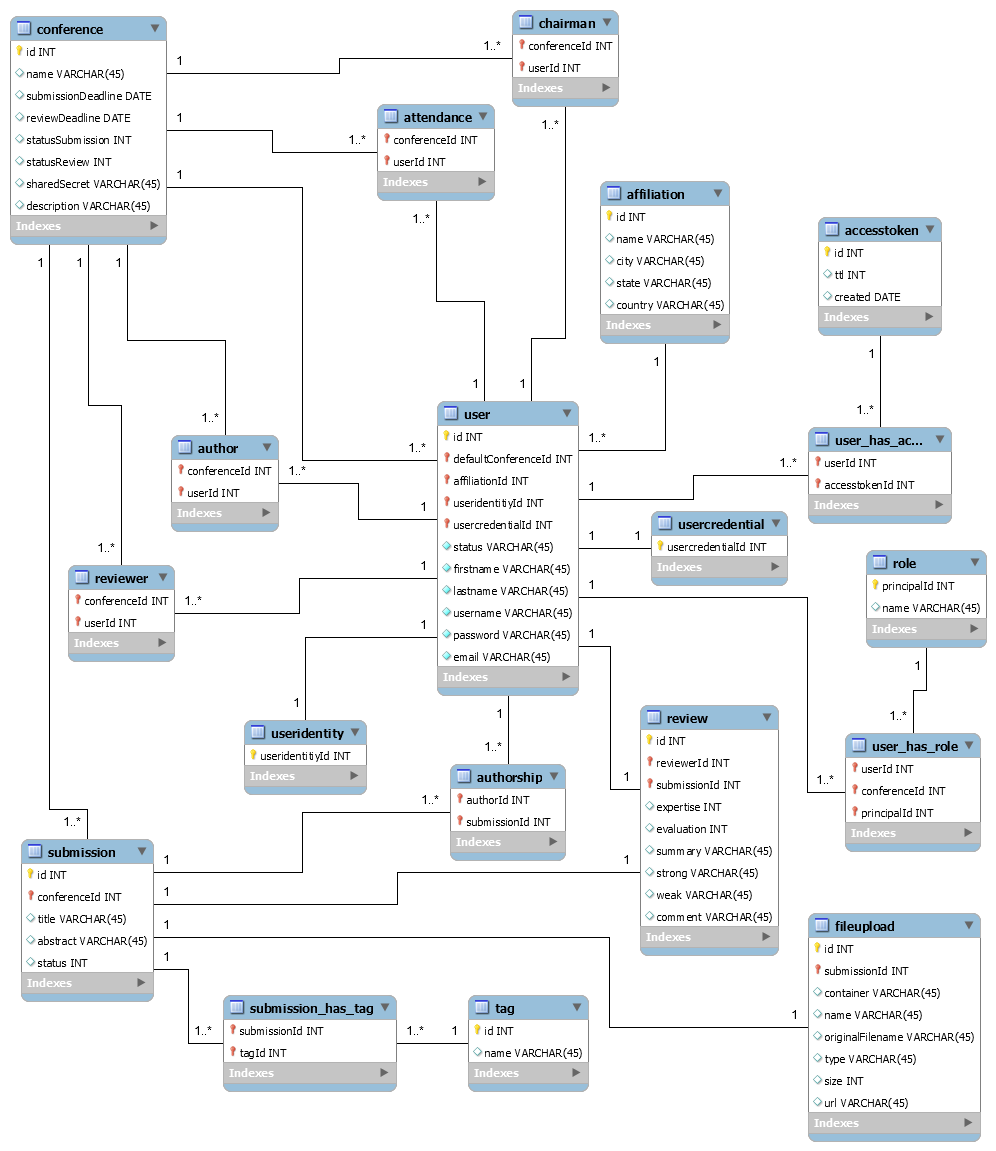
\includegraphics[width=\textwidth]{img/er-diagram}
            \caption{The entity relationship model of the application's database.}
            \label{fig:appendix:erm:er-diagram}
        \end{figure}

    \clearpage

  \chapter{Application Screenshots}
  \label{ch:appendix:screenshots}

        \begin{figure}[!ht]
            \centering
            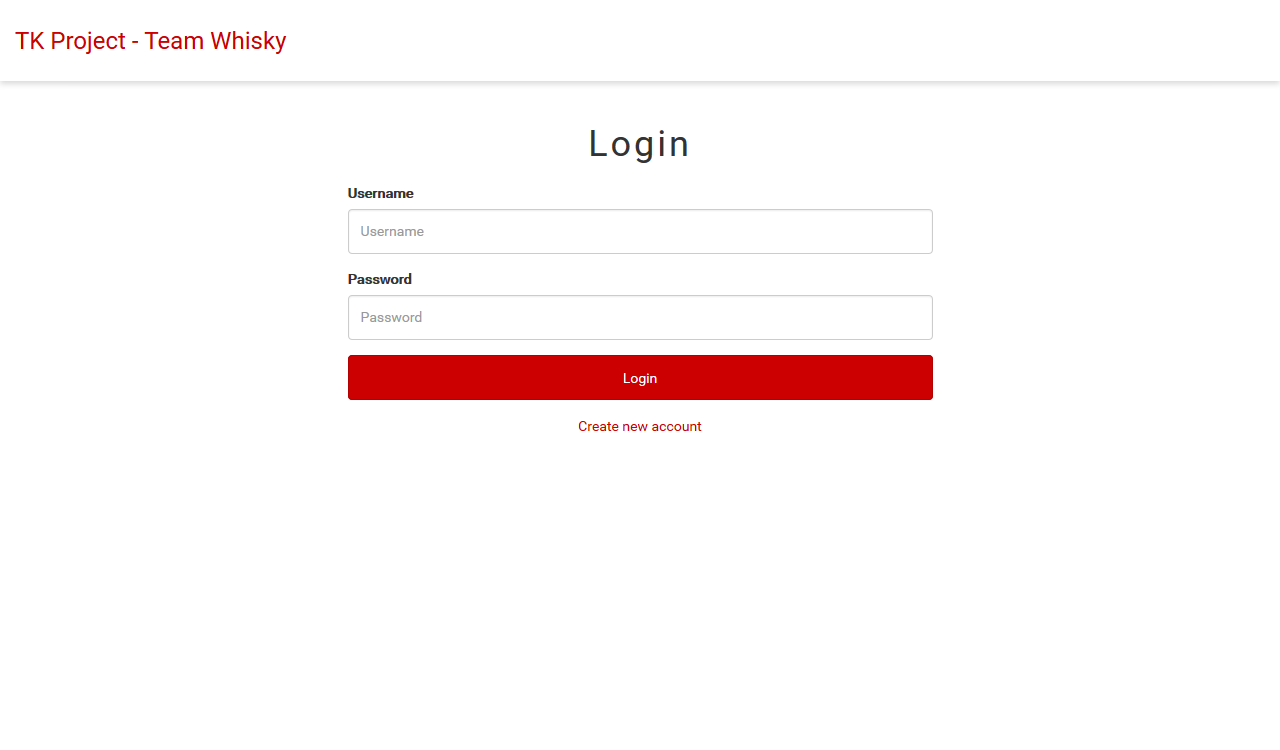
\includegraphics[width=\textwidth]{img/ui-login}
            \caption{Login page}
            \label{fig:appendix:screenshots:ui-login}
        \end{figure}

        \begin{figure}[!ht]
            \centering
            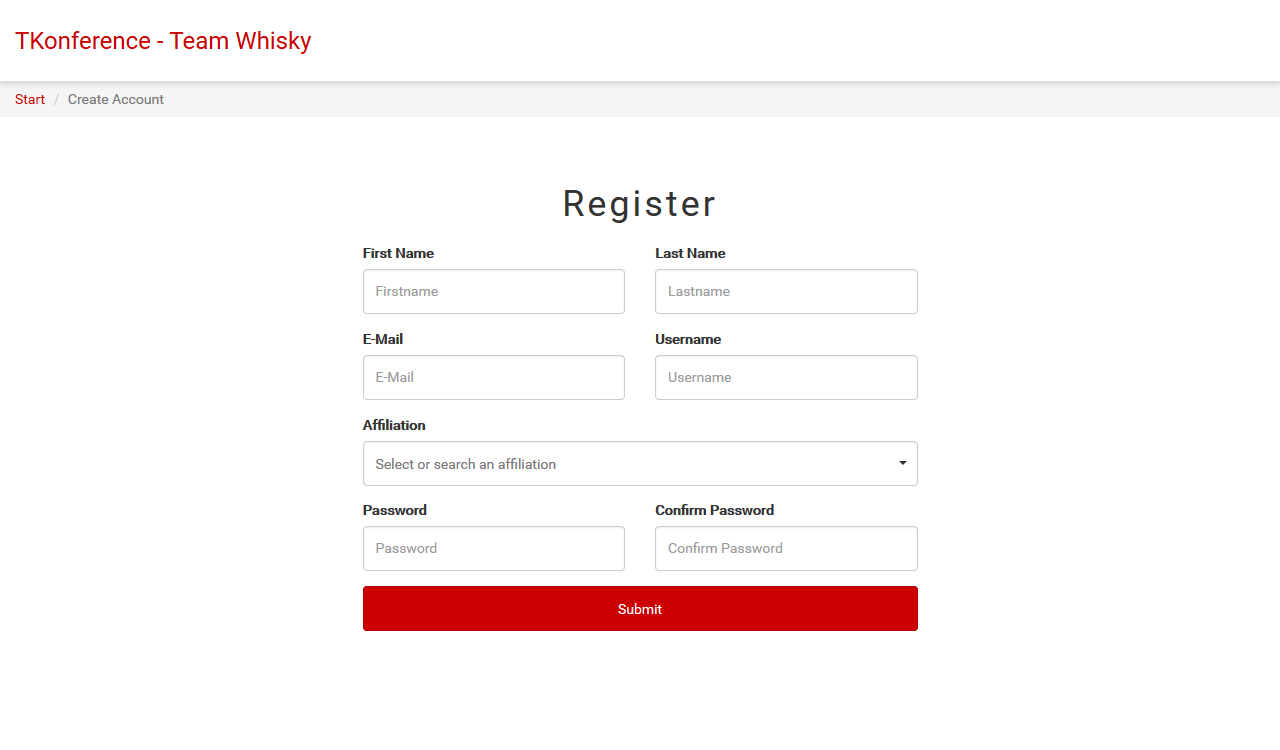
\includegraphics[width=\textwidth]{img/ui-register}
            \caption{Register page. Affiliation field is pre-populated with a list of known universities (\textasciitilde300).}
            \label{fig:appendix:screenshots:ui-register}
        \end{figure}

        \begin{figure}[!ht]
            \centering
            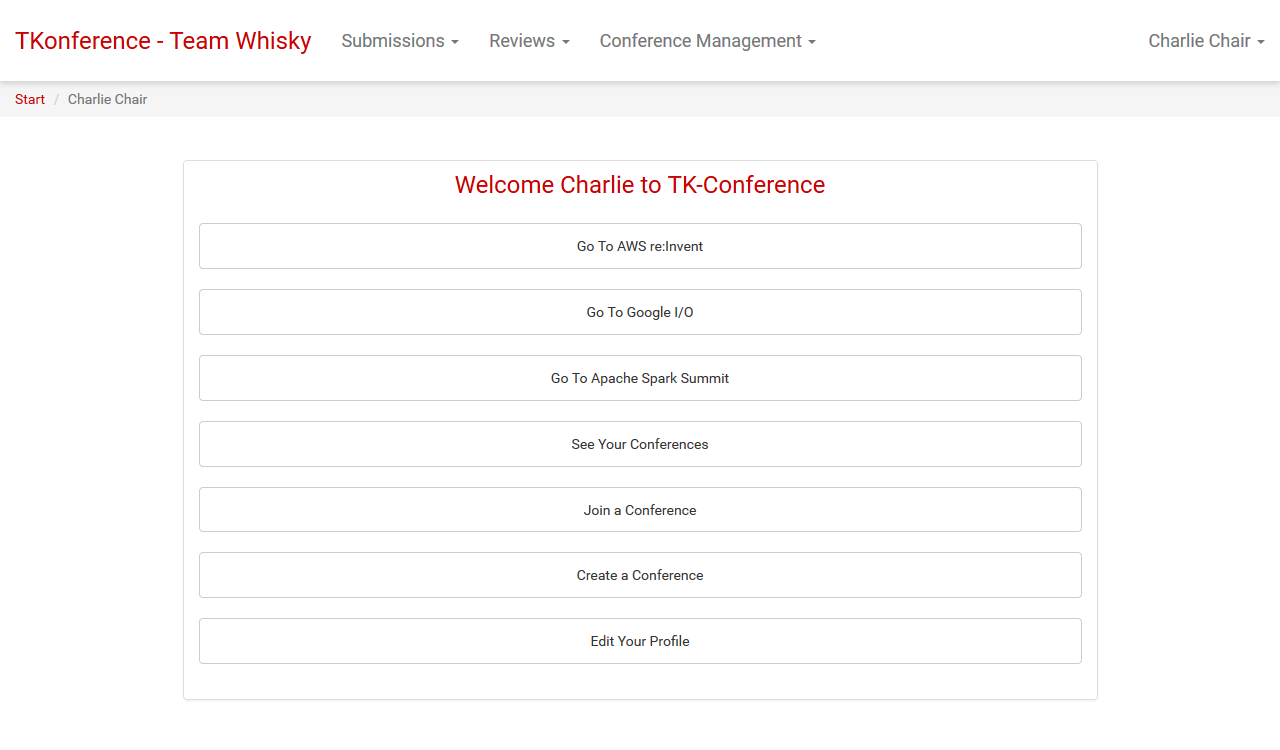
\includegraphics[width=\textwidth]{img/ui-account-home}
            \caption{Account overview. Provides important quick links}
            \label{fig:appendix:screenshots:ui-account-home}
        \end{figure}

        \begin{figure}[!ht]
            \centering
            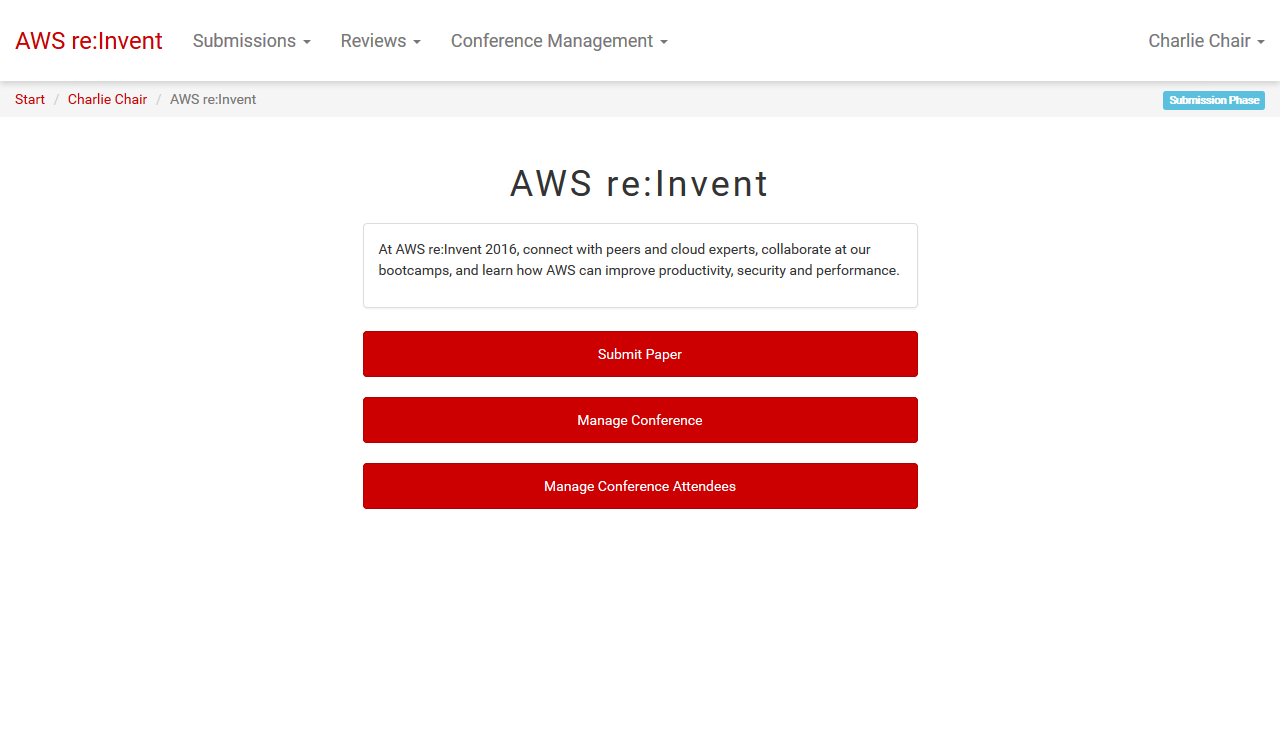
\includegraphics[width=\textwidth]{img/ui-conference-home}
            \caption{Conference overview. Provides some quick links according to the user permissions.}
            \label{fig:appendix:screenshots:ui-conference-home}
        \end{figure}

        \begin{figure}[!ht]
            \centering
            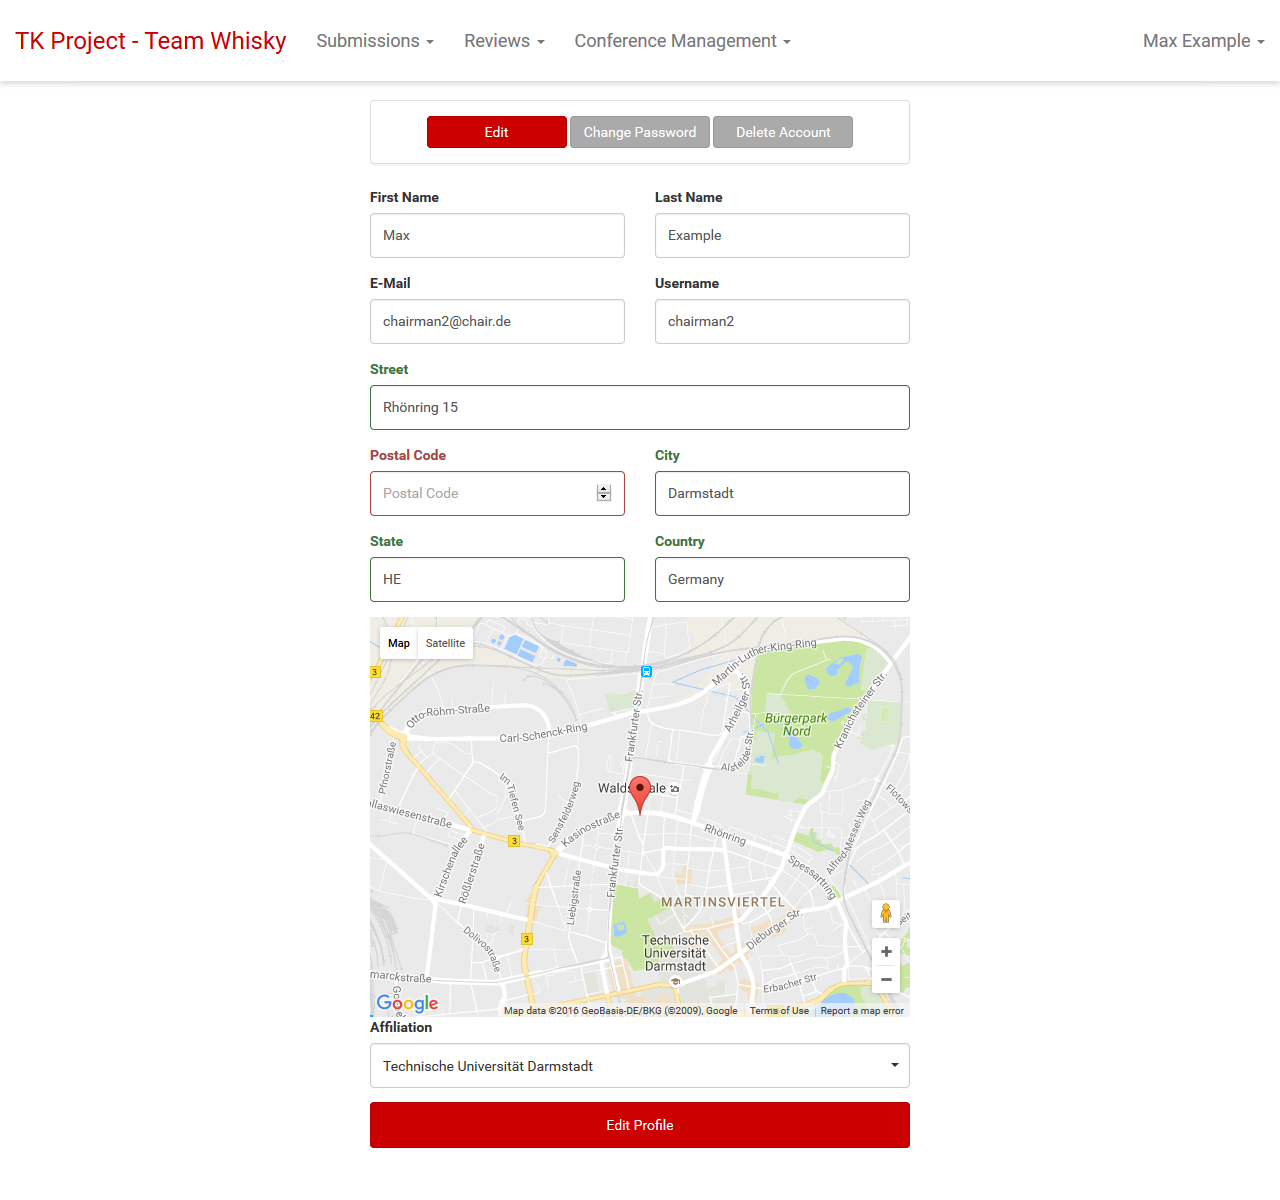
\includegraphics[width=\textwidth]{img/ui-manage-profile}
            \caption{Manage profile. Allows the user to edit his profile, change his password, and delete is account.}
            \label{fig:appendix:screenshots:ui-manage-profile}
        \end{figure}

        \begin{figure}[!ht]
            \centering
            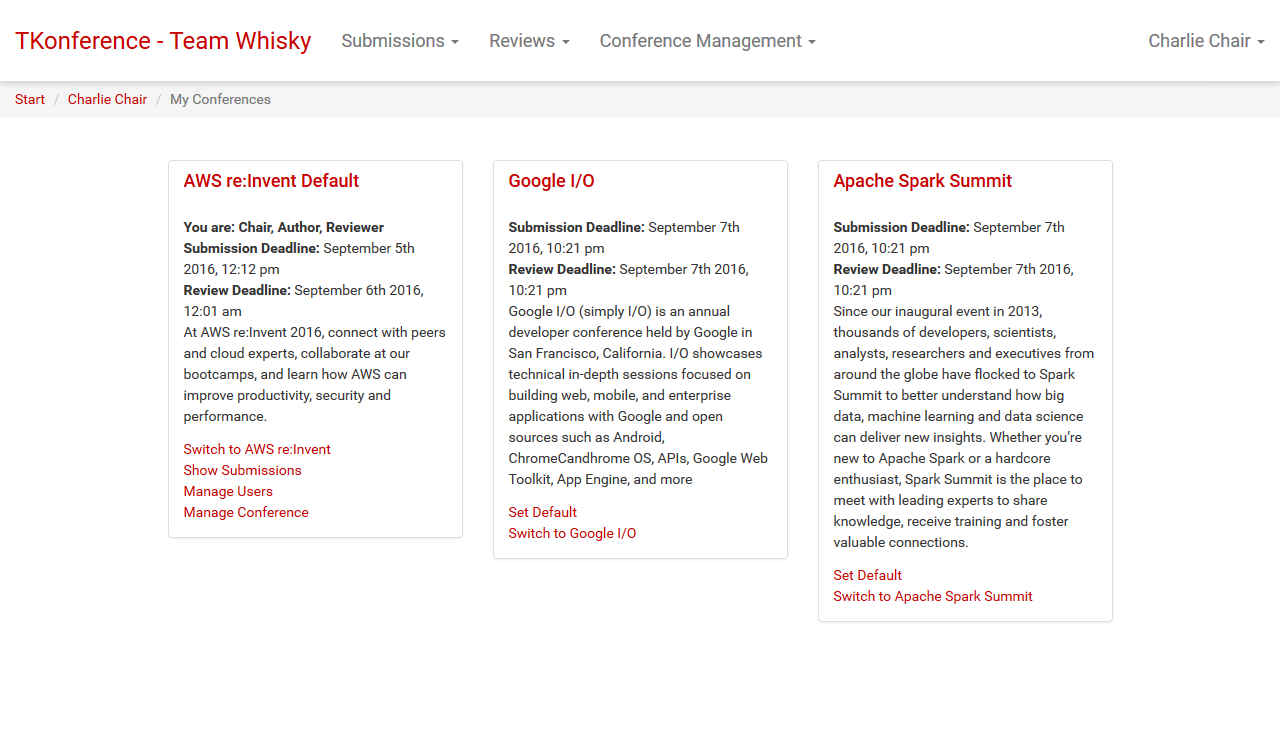
\includegraphics[width=\textwidth]{img/ui-list-conferences}
            \caption{List attended conferences. Provides some quick links according to the user permissions.}
            \label{fig:appendix:screenshots:ui-list-conferences}
        \end{figure}

        \begin{figure}[!ht]
            \centering
            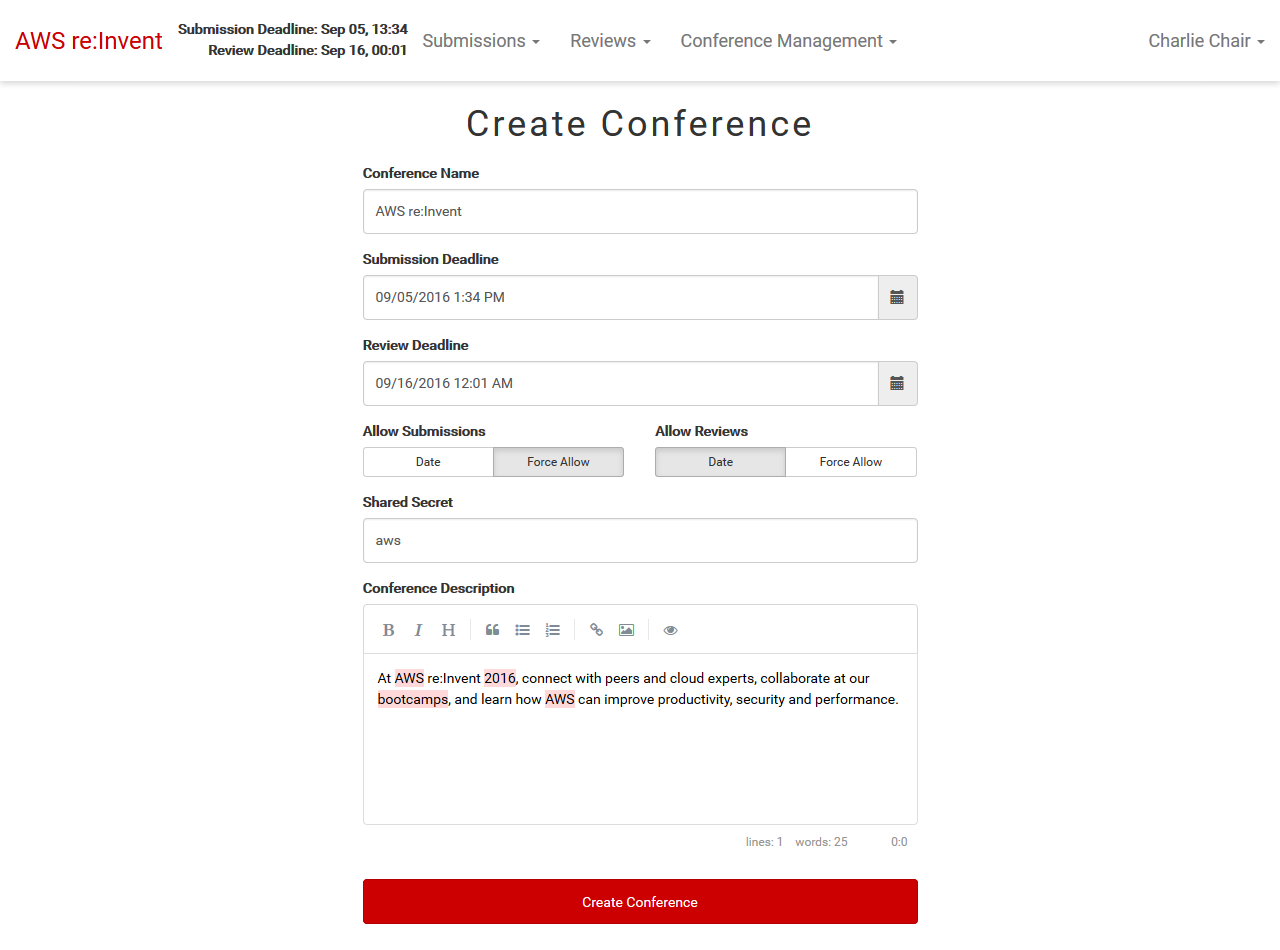
\includegraphics[width=\textwidth]{img/ui-conference-create}
            \caption{Conference creation. Allows to set the name, description and deadlines of a conference. The submission and review phase can be force opened to allow submissions/reviews outside of the defined intervals. The shared secret is used by attendees to join the conference.}
            \label{fig:appendix:screenshots:ui-conference-create}
        \end{figure}

        \begin{figure}[!ht]
            \centering
            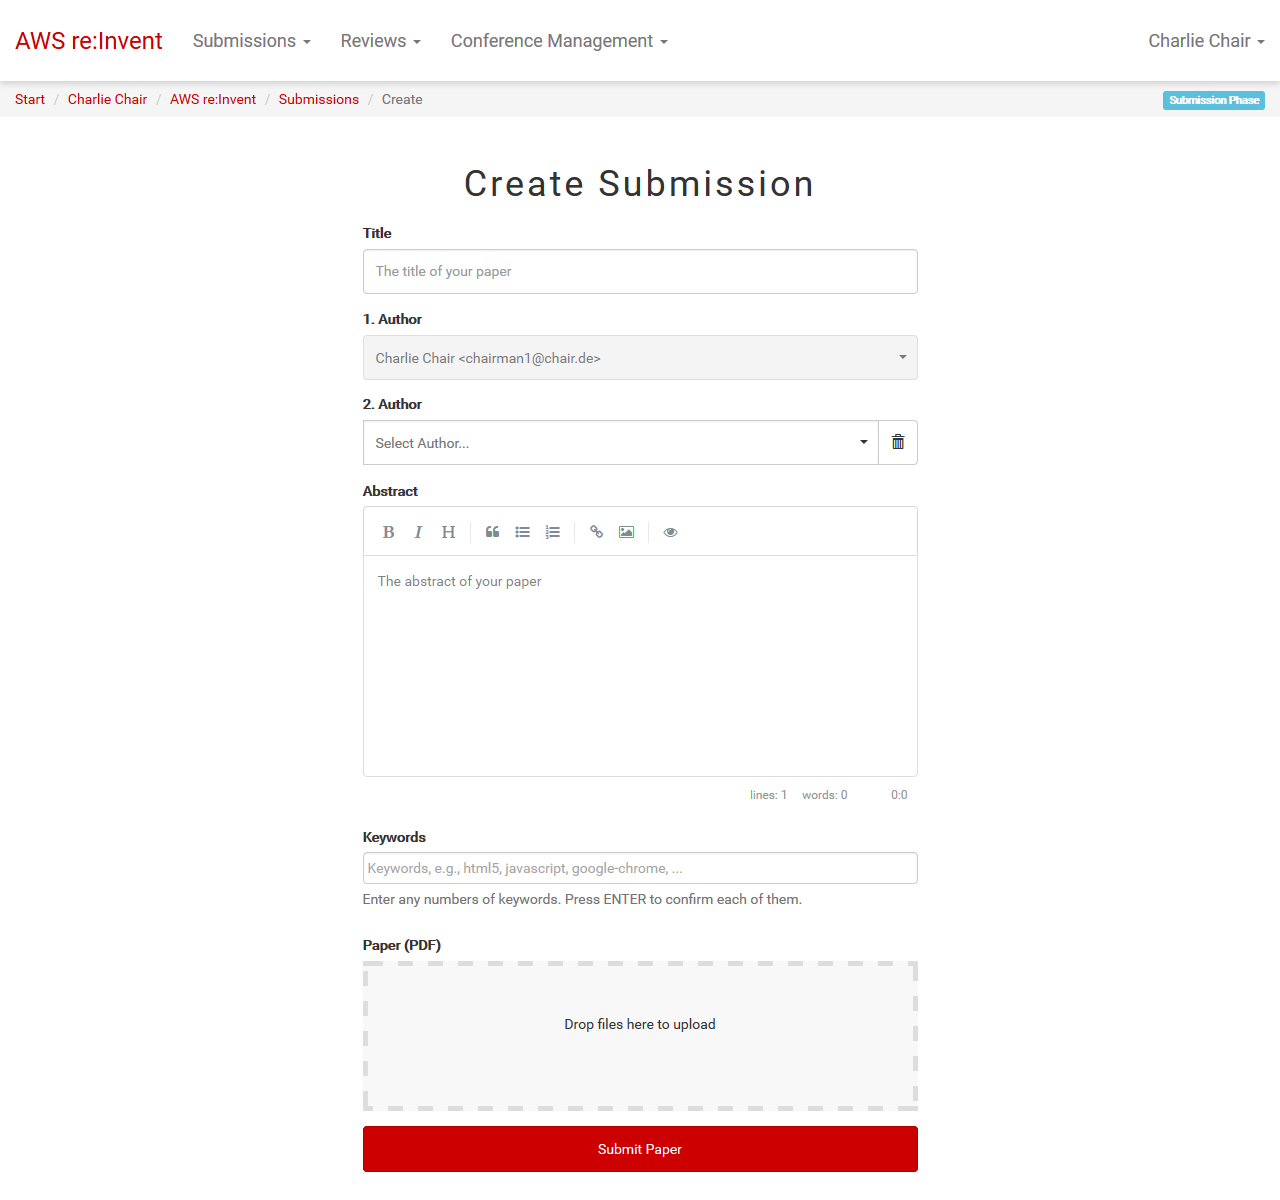
\includegraphics[width=\textwidth]{img/ui-submission-create}
            \caption{Submission creation. Allows to select multiple authors from the list of conference attendees. The abstract supports markdown syntax. Keywords are auto-suggested and created on-the-fly. Paper must be provided as PDF.}
            \label{fig:appendix:screenshots:ui-submission-create}
        \end{figure}

        \begin{figure}[!ht]
            \centering
            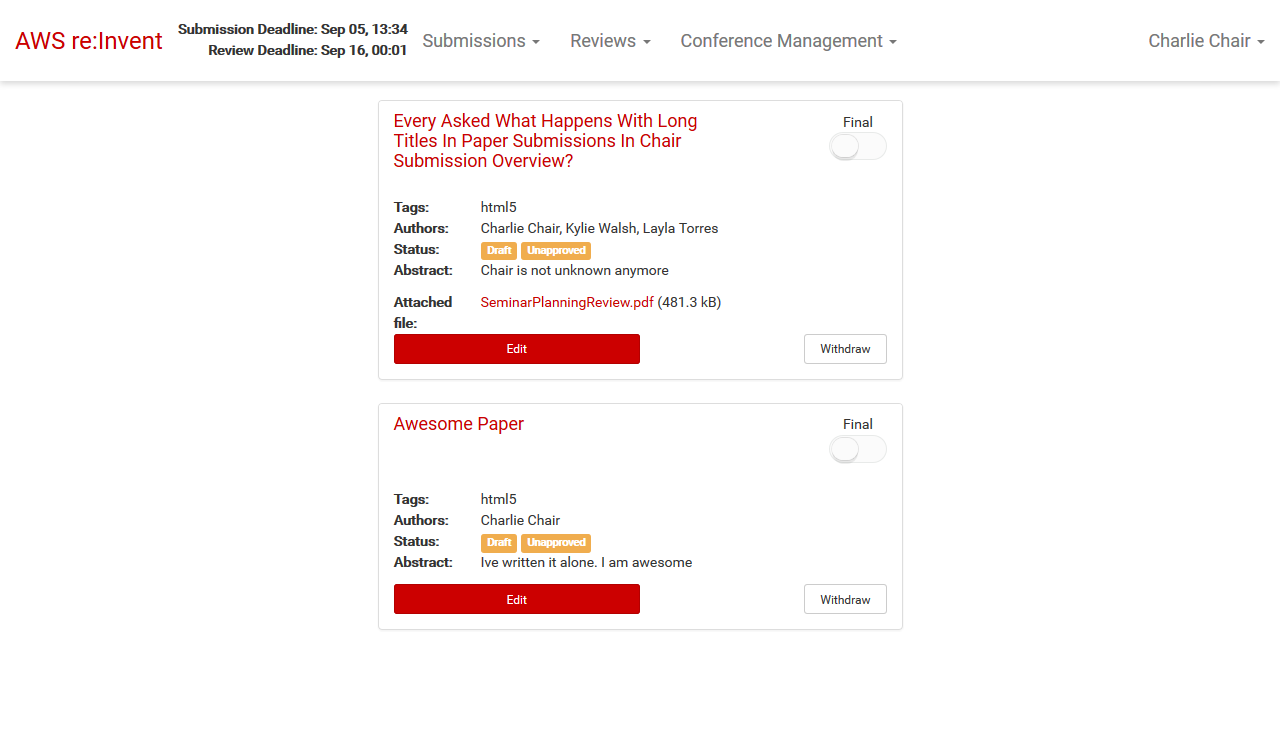
\includegraphics[width=\textwidth]{img/ui-submission-overview}
            \caption{Submission overview. Lists created submissions and shows a summary and the current status. The user can choose to finalize the submission which allows reviewers to review the submission early on.}
            \label{fig:appendix:screenshots:ui-submission-overview}
        \end{figure}

        \begin{figure}[!ht]
            \centering
            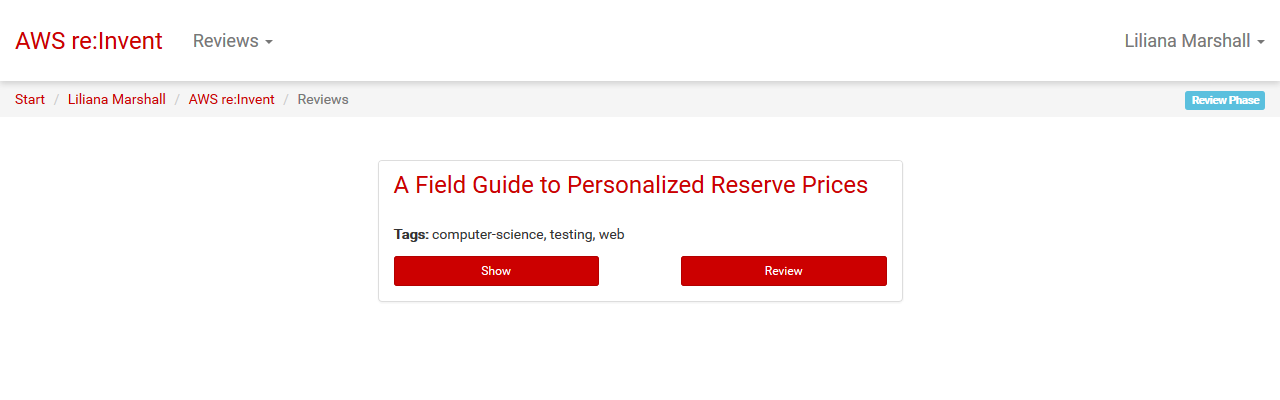
\includegraphics[width=\textwidth]{img/ui-review-overview}
            \caption{Review overview. Lists reviews of assigned submissions and allows to edit them during the review phase.}
            \label{fig:appendix:screenshots:ui-review-overview}
        \end{figure}

        \begin{figure}[!ht]
            \centering
            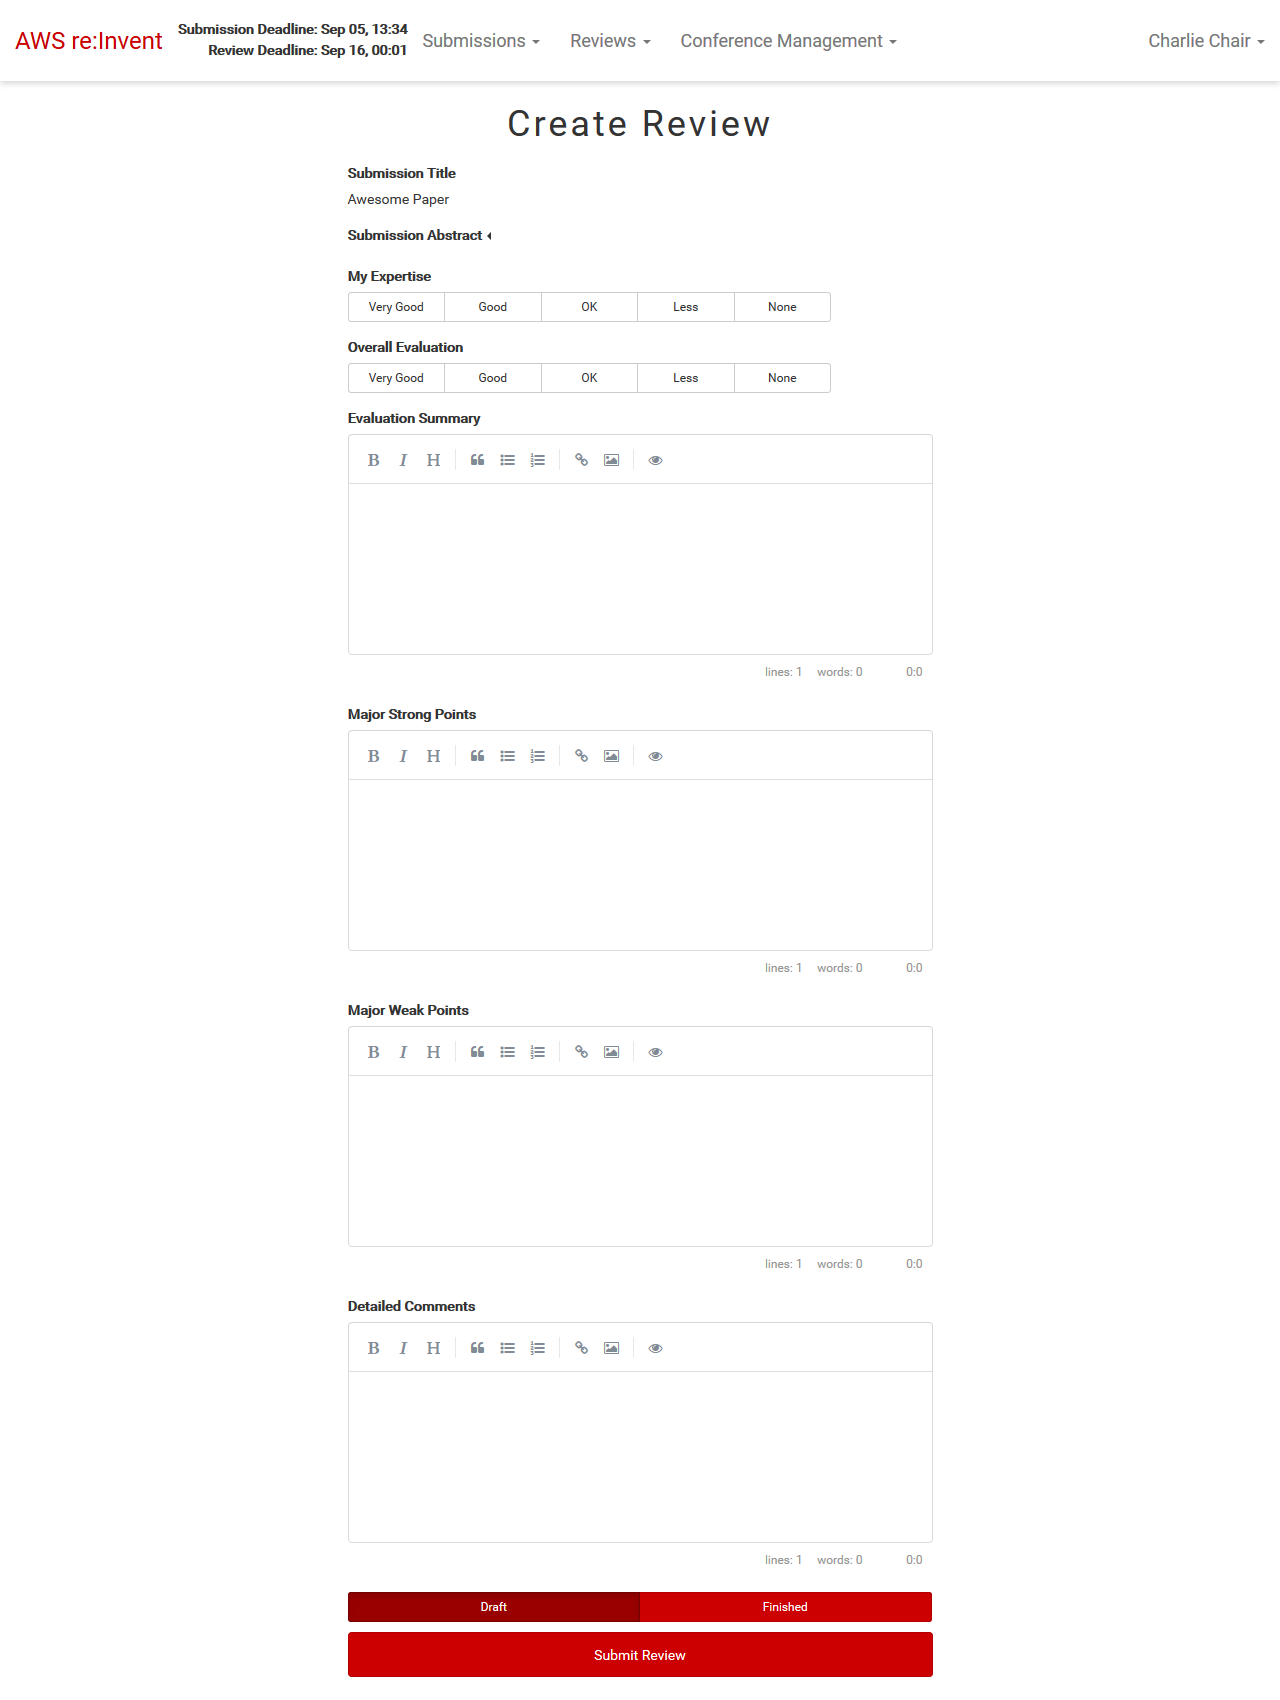
\includegraphics[width=\textwidth]{img/ui-review-create}
            \caption{Review creation. Allows for an abstract rating and textual feedback (markdown support).}
            \label{fig:appendix:screenshots:ui-review-create}
        \end{figure}

        \begin{figure}[!ht]
            \centering
            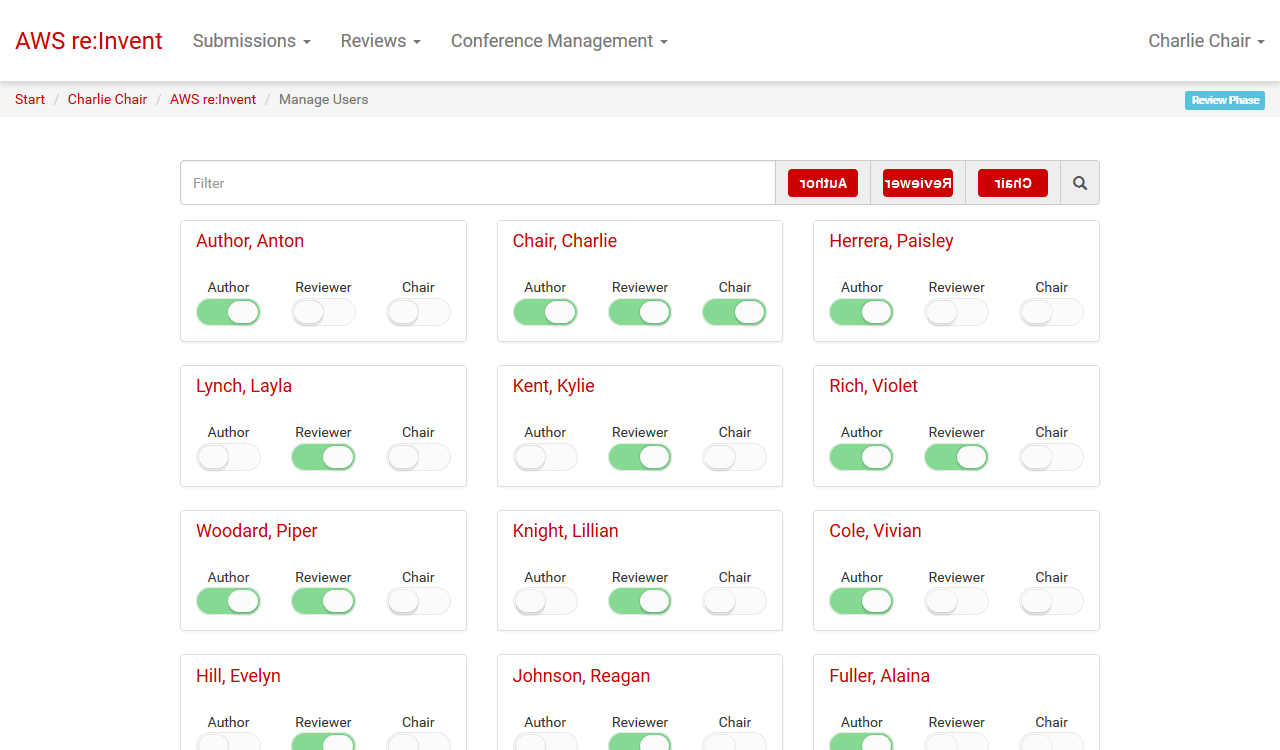
\includegraphics[width=\textwidth]{img/ui-user-role-assignment}
            \caption{Role Assignment. Allows the chair to manage the roles of the conference attendees. The filter on top allows to filter for attendees that have a specific role or name.}
            \label{fig:appendix:screenshots:ui-user-role-assignment}
        \end{figure}

        \begin{figure}[!ht]
            \centering
            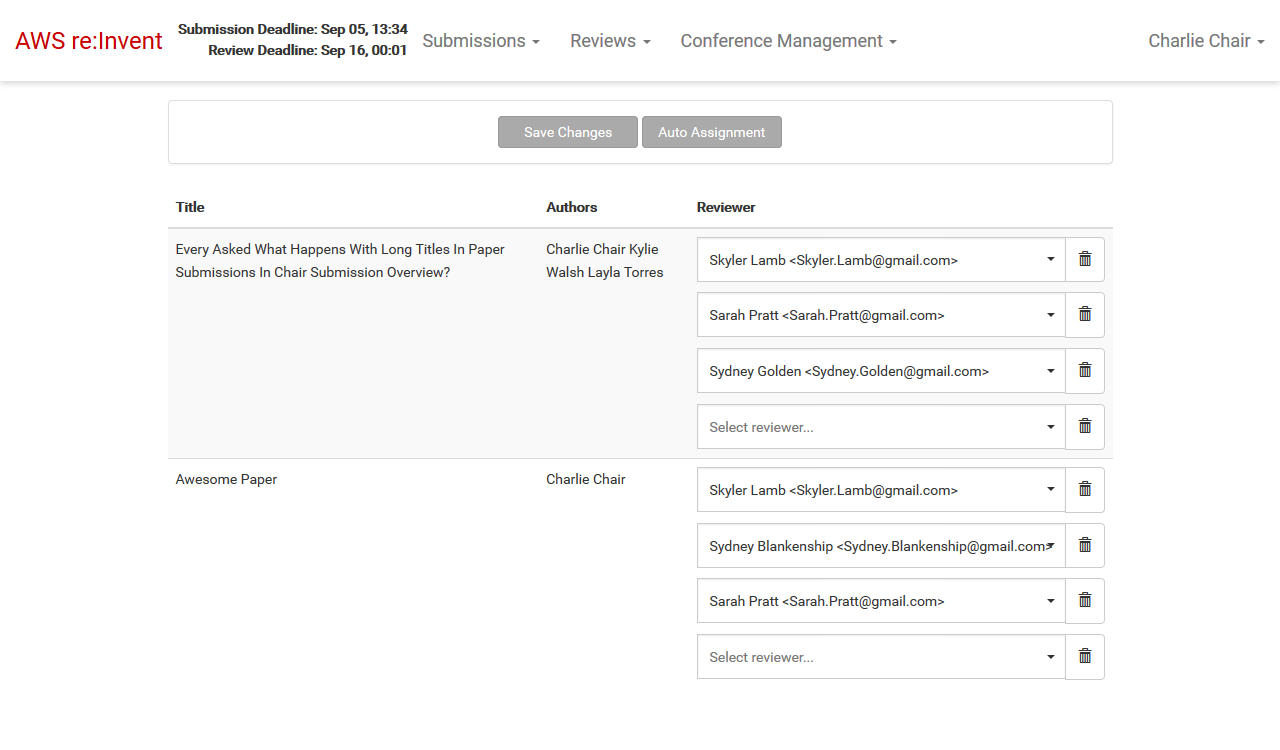
\includegraphics[width=\textwidth]{img/ui-reviewer-assignment}
            \caption{Reviewer Assignment. Allows the chair to assign one or more reviewers to a submission. This can be done either manually or automatically, or in a hybrid approach.}
            \label{fig:appendix:screenshots:ui-reviewer-assignment}
        \end{figure}

        \begin{figure}[!ht]
            \centering
            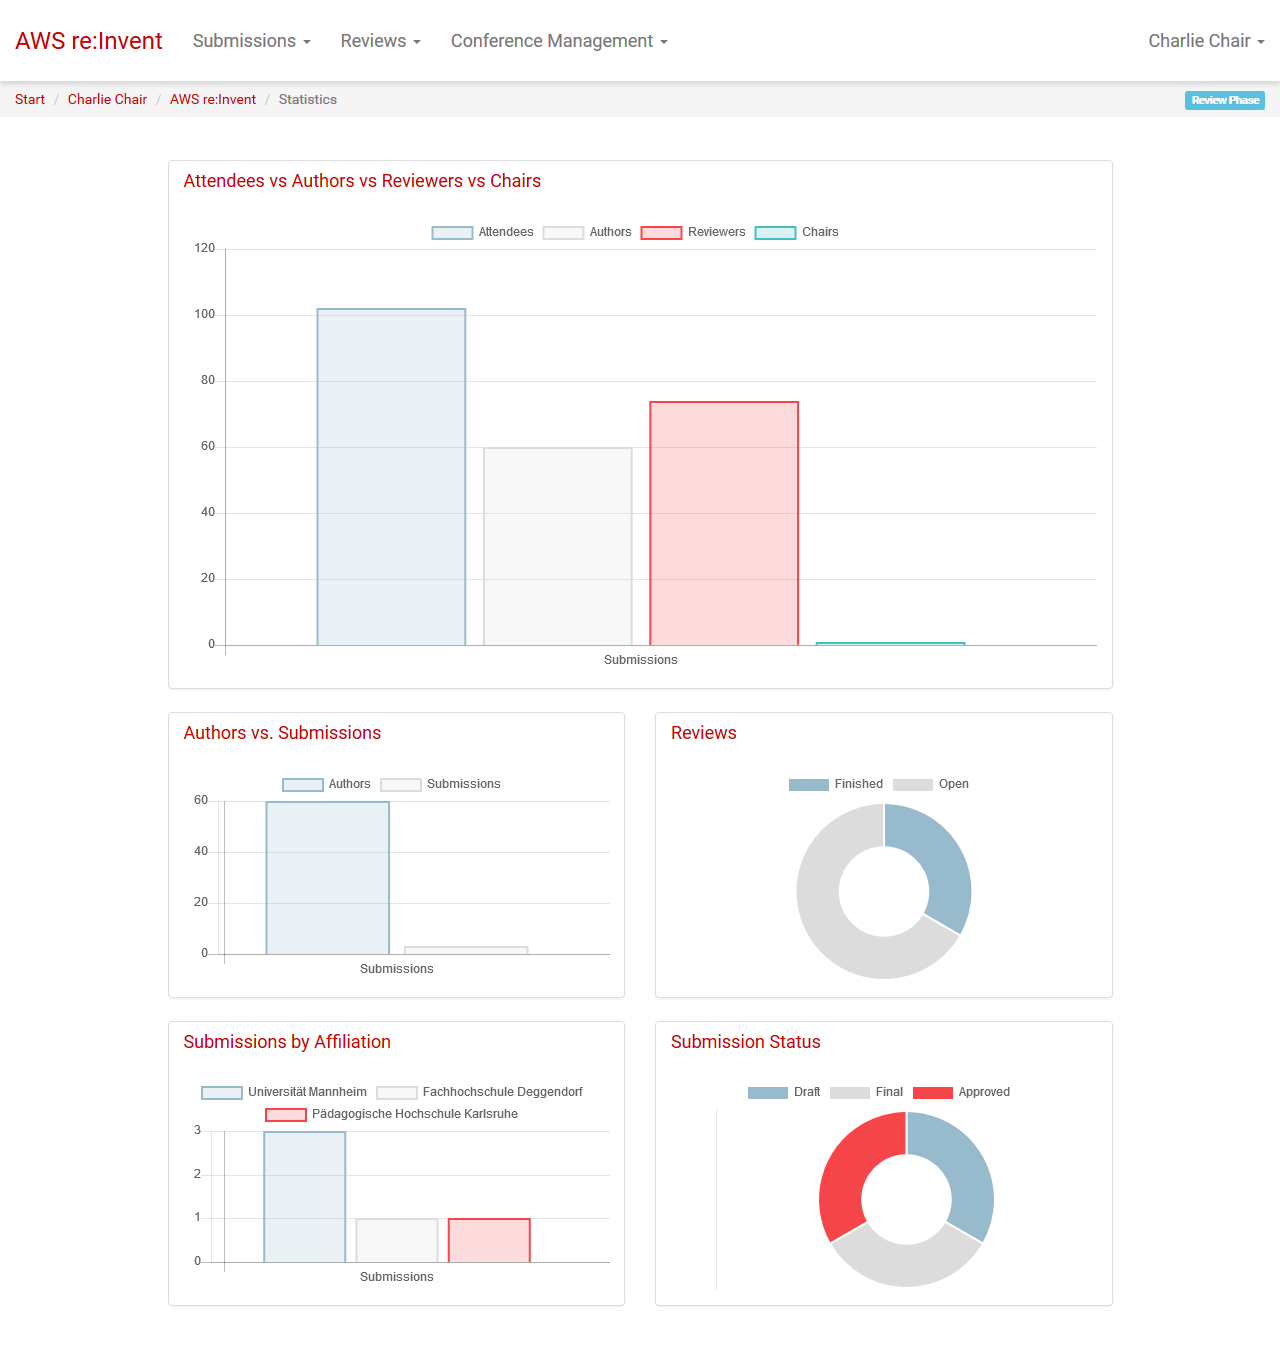
\includegraphics[width=\textwidth]{img/ui-statistics}
            \caption{Conference Statistics. See \ref{ch:user:chair:statistics} for more information on the different statistics.}
            \label{fig:appendix:screenshots:ui-statistics}
        \end{figure}

    % Ensure to keep figures grouped together
    \clearpage

  \chapter{(Un)Implemented Features}
  \label{ch:appendix:features}

    % List of features goes here
    Below is the list of (un)implemented features, copied from the SCM wiki page.%
    \footnote{\url{https://scm.informatik.tu-darmstadt.de/projects/iptk-ss2016/wiki/Conference_management_system_-_Features}}
    A checked box ($\boxtimes$) means that the feature is implemented whereas an unchecked box ($\square$) means that the feature is (partly) unimplemented
        \begin{itemize}
            \setlength\itemsep{0em}
            \item Roles
            \begin{itemize}
                \item[$\boxtimes$] Authors [0..*]
                \item[$\boxtimes$] Reviewers [0..*]
                \item[$\boxtimes$] Chair [1..*]
            \end{itemize}

            \item General
            \begin{itemize}
                \item[$\boxtimes$] responsive design: access the web application with different kinds of devices (mobile, tablet, pc..)
            \end{itemize}

            \item As a user, I can
            \begin{itemize}
                \item[$\boxtimes$] register to the system at least with email, password
                \begin{itemize}
                    \item[$\boxtimes$] emails are unique
                    \item[$\boxtimes$] users can have multiple roles (e.g., author and reviewer)
                    \item[$\boxtimes$] additional information (see slides)
                    \begin{itemize}
                        \item[$\boxtimes$] e.g., basic profile (given name, family name, postal address)
                        \item[$\boxtimes$] e.g., affiliation (institution, city, state, country)
                    \end{itemize}
                \end{itemize}
                \item[$\boxtimes$] login to the system at least with registered email, password
                \item[$\boxtimes$] edit my profile (password, additional information)
                \item[$\boxtimes$] remove my profile
                \item[$\boxtimes$] logout
            \end{itemize}

            \item As a author, I can
            \begin{itemize}
                \item[$\boxtimes$] create a new submission (if submission is open)
                \begin{itemize}
                    \item[$\boxtimes$] title
                    \item[$\boxtimes$] registered authors [1..*] (given name, family name, email affiliation)
                    \item[$\boxtimes$] abstract
                    \item[$\boxtimes$] keywords (multi-selection) that describe the submission (e.g., research fields)
                    \item[$\boxtimes$] upload the paper (.pdf)
                \end{itemize}
                \item[$\boxtimes$] access current submissions (overview)
                \begin{itemize}
                    \item[$\boxtimes$] status: incompleted, completed, closed, accepted, rejected
                \end{itemize}
                \item[$\boxtimes$] look at a submission
                \item[$\boxtimes$] edit a submission (if submission is open)
                \item[$\boxtimes$] withdraw a submission
            \end{itemize}

            \item As a reviewer, I can
            \begin{itemize}
                \item[$\boxtimes$] access assigned submissions (overview + status)
                \item[$\boxtimes$] look at an assigned submission
                \begin{itemize}
                    \item[$\boxtimes$] details, pdf download or view
                \end{itemize}
                \item[$\boxtimes$] make a review > template (if review is open)
                \begin{itemize}
                    \item[$\boxtimes$] reviewer expertise: (1) not familar w/ the topic - (5) expert
                    \item[$\boxtimes$] overall evaluation: (1) strong reject - (5) strong accept
                    \item[$\boxtimes$] summary
                    \item[$\boxtimes$] major strong popints
                    \item[$\boxtimes$] major weak points
                    \item[$\boxtimes$] detailed comments
                \end{itemize}
                \item[$\boxtimes$] edit a review (if reviewing phase is open)
            \end{itemize}

            \item As a chair, I can
            \begin{itemize}
                \item[$\boxtimes$] list all paper submissions
                \begin{itemize}
                    \item[$\boxtimes$] look at a submissions (details, pdf download or view)
                    \item[$\boxtimes$] withdraw a submission
                \end{itemize}
                \item[$\boxtimes$] list all authors
                \begin{itemize}
                    \item[$\boxtimes$] look at detail information
                \end{itemize}
                \item[$\boxtimes$] list all reviewers
                \begin{itemize}
                    \item[$\boxtimes$] look at detail information
                \end{itemize}
                \item[$\boxtimes$] list all reviews
                \begin{itemize}
                    \item[$\boxtimes$] look at a review
                \end{itemize}
                \item[$\boxtimes$] assign papers to reviewers
                \begin{itemize}
                    \item[$\boxtimes$] conflict avoidance: an author is not allow to review his own paper
                \end{itemize}
                \item[$\boxtimes$] do the schedule management
                \begin{itemize}
                    \item[$\boxtimes$] automatic: set close deadlines for submissions and reviews
                    \item[$\boxtimes$] manual: (re-)open/close submissions and reviews
                \end{itemize}
                \item[$\boxtimes$] view fancy summary charts or reports (e.g., total submission, acceptances, topics, countries etc.)
            \end{itemize}

            \item Bonus features (OPTIONAL)
            \begin{itemize}
                \item[$\square$] users must confirm their registration by clicking on a registration link sent via email
                \item[$\square$] email notification to submitters and reviewers (status changes)
                \item[$\square$] chat with other online authors
                \item[$\boxtimes$] automatic assignment (even distribution) and conflict resolving
                \item[$\boxtimes$] a user can create multiple conference events and becomes the chair (=administrator) of them%
                \footnote{Implementing this feature sadly broke the server side ACL mechanisms. In \texttt{LoopBack}, ACL roles can only be defined globally, i.e. a user can either have the role \texttt{chair} or not, but not selectively for only some database records. We noted this after implementing this bonus feature and decided to leave it as is. This means that server side access checks are currently not working and a workaround must be found when used in production mode.}
            \end{itemize}
        \end{itemize}

\end{document}
